\documentclass[a4paper, 14pt]{extreport}
\usepackage{cmap}
\usepackage{amssymb}
\usepackage{amsmath}
\usepackage{graphicx}
\usepackage{amsthm}
\usepackage{upgreek}
\usepackage{listings}
\usepackage{setspace}
\usepackage{booktabs}
\numberwithin{equation}{subsection}
\usepackage[T2A]{fontenc}
\usepackage[utf8]{inputenc}
\usepackage[normalem]{ulem}
\usepackage{mathtext} % русские буквы в формулах
\usepackage[left=3cm,right=1.5cm,top=2cm,bottom=2cm]{geometry}
\usepackage{linegoal}
\usepackage[english,russian]{babel}
\usepackage[unicode]{hyperref}
\usepackage{indentfirst}
\setlength{\parindent}{1cm} % Настройка длины красной строки (например, 1.25 см)
%\usepackage{pythonhighlight}

\usepackage{titlesec}
\usepackage{caption}
\usepackage{multirow}

\newcommand{\specialcell}[2][c]{%
	\begin{tabular}[#1]{@{}c@{}}#2\end{tabular}}

% Настройка заголовков для таблиц
\captionsetup[table]{labelsep=space}
\addto\captionsrussian{\renewcommand{\tablename}{\bfseries Таблица}}
% chapter settings
\titleformat{\chapter}[display]
{\centering\large\bfseries}{\chaptertitlename\ \thechapter}{0pt}{\large}   
\titlespacing*{\chapter}{5pt}{-20pt}{18pt}
\titlespacing*{\section}{0pt}{18pt}{18pt} 
\titlespacing*{\subsection}{0pt}{18pt}{18pt} 
\titlespacing*{\subsubsection}{0pt}{5pt}{5pt} 
% section settings
\titleformat{\section}[block]
{\raggedright\large\bfseries}
{\hspace{1.25cm}\thesection\ }{0pt}{}
\titleformat{\subsection}[block]
{\raggedright\large\bfseries}
{\hspace{1.25cm}\thesubsection\ }{0pt}{}
\titleformat{\subsubsection}
{\raggedright\normalfont\normalsize\bfseries} % Шрифт для подподсекции
{\thesubsubsection\hspace{0.5em}} % Номер подподсекции с пробелом
{0pt} % Отступ от номера
{\hspace{1.25cm}}
\addto\captionsrussian{% Replace "english" with the language you use
	\renewcommand{\contentsname}%
	{\centering \large ОГЛАВЛЕНИЕ}%
	\renewcommand{\chaptername}{ГЛАВА}
	\renewcommand{\chaptertitlename}{ГЛАВА}
	\renewcommand{\bibname}{\large СПИСОК ИСПОЛЬЗОВАННОЙ ЛИТЕРАТУРЫ}
}


\newcommand\Norm[1]{\left\| #1 \right\|}
\newcommand{\dif}{\mathrm{d}}
\newcommand{\Rm}{\mathbb{R}}
\newcommand{\Cm}{\mathbb{C}}
\newcommand{\Z}{\mathbb{Z}}
\newcommand{\I}{\mathbb{I}}
\newcommand{\N}{\mathbb{N}}
\newcommand{\rank}{\operatorname{rank}}
\newcommand{\Ra}{\Rightarrow}
\newcommand{\ra}{\rightarrow}
\newcommand{\FI}{\Phi}
\newcommand{\Sp}{\text{Sp}}
\renewcommand{\leq}{\leqslant}
\renewcommand{\geq}{\geqslant}
\renewcommand{\alpha}{\upalpha}
\renewcommand{\beta}{\upbeta}
\renewcommand{\gamma}{\upgamma}
\renewcommand{\delta}{\updelta}
\renewcommand{\varphi}{\upvarphi}
\renewcommand{\tau}{\uptau}
\renewcommand{\theta}{\uptheta}
\renewcommand{\lambda}{\uplambda}
\renewcommand{\psi}{\uppsi}
\renewcommand{\mu}{\upmu}
\renewcommand{\omega}{\upomega}
\renewcommand{\d}{\partial}
\renewcommand{\xi}{\upxi}
\renewcommand{\epsilon}{\upvarepsilon}
\newcommand{\cov}{\operatorname{cov}}
\newcommand{\E}{\mathbb E}
\newcommand{\Var}{\operatorname{Var}}
\newcommand{\const}{\operatorname{const}}
\numberwithin{equation}{section}
\newtheorem*{theorem}{Теорема}
\newtheorem*{cor}{Следствие}
\newtheorem*{lem}{Лемма}
\usepackage{stackengine}

% Переоформление некоторых стандартных названий


\begin{document}
	\def\contentsname{ОГЛАВЛЕНИЕ}
	
	% Оформление титульного листа
	\begin{titlepage}
		\begin{center}
			\textsc{МИНИСТЕРСТВО ОБРАЗОВАНИЯ РЕСПУБЛИКИ БЕЛАРУСЬ БЕЛОРУССКИЙ ГОСУДАРСТВЕННЫЙ УНИВЕРСИТЕТ
				\\[5mm]
				ФАКУЛЬТЕТ ПРИКЛАДНОЙ МАТЕМАТИКИ И ИНФОРМАТИКИ\\[2mm]
				Кафедра математического моделирования и анализа данных
			}
			
			\vfill
			
			\textbf{Курсовой проект
				\\[3mm]
				«Краткосрочное прогнозирование и наукастинг макроэкономических временных рядов на основе векторных моделей авторегрессии по смешанным данным»
				\\[26mm]
			}
		\end{center}
		
		\hfill
		\begin{minipage}{.5\textwidth}
			\begin{flushright}
				Бовта Тимофея Анатольевича\\
				студента 4 курса 7 группы\\
				специальности «прикладная математика»\\[5mm]
				
				Научный руководитель:\\[2mm] 
				В. И. Малюгин\\
				зав. кафедрой ММАД,\\
				доктор экономических наук,\\
				доцент
			\end{flushright}
		\end{minipage}%
		\vfill
		\begin{center}
			Минск, 2024\ г.
		\end{center}
	\end{titlepage}
	\newpage
	\setcounter{page}{2}
	\begin{center}
		\bf
		{
			\setstretch{0.9}
			\small\mbox{МИНИСТЕРСТВО~ОБРАЗОВАНИЯ~РЕСПУБЛИКИ~БЕЛАРУСЬ} \\~\\
			\mbox{БЕЛОРУССКИЙ~ГОСУДАРСТВЕННЫЙ~УНИВЕРСИТЕТ} \\~\\
			\mbox{ФАКУЛЬТЕТ~ПРИКЛАДНОЙ МАТЕМАТИКИ~И~ИНФОРМАТИКИ} \\~\\
			\mbox{Кафедра~математического~моделирования~и~анализа~данных} \\~\\[2mm]
		}
		\bf
		{
			\mbox{\small ЗАДАНИЕ}\\
			\mbox{\small НА КУРСОВОЙ ПРОЕКТ} \\[6mm]
		}
	\end{center}
	\small{    Студент \quad Бовт Тимофей Анатольевич\\[2mm]
		1. Тема курсового проекта\\
		<<КРАТКОСРОЧНОЕ ПРОГНОЗИРОВАНИЕ И НАУКАСТИНГ МАКРОЭКОНОМИЧЕСКИХ ВРЕМЕННЫХ РЯДОВ НА ОСНОВЕ ВЕКТОРНЫХ МОДЕЛЕЙ АВТОРЕГРЕССИИ ПО СМЕШАННЫМ ДАННЫМ>>.\\[6mm]
		2. Исходные данные к курсовому проекту
		
		2.1. Малюгин В. И. Краткосрочное прогнозирование и наукастинг темпов роста инфляции на основе моделей по смешанным данным --- Журнал <<Банковский вестник>> №1/726 --- С. 23-36.
		
		2.2. Макеева, Н.М. Наукастинг элементов использования ВВП России / Н.М. Макеева, И.П. Станкевич -- Статья 2022/10, Экономический журнал ВШЭ.
		
		2.3. Макеева, Н.М. Наукастинг макроэкономических показателей экономики России на основе анализа новостного фона и регулярных данных Росстата / Н. М. Макеева, И. П. Станкевич\\[2mm]
		3. Перечень подлежащих разработке вопросов:
		
		3.1. Провести обзор по теме <<Проблема краткосрочного прогнозирования и наукастинга для данных смешанной частоты>>.
		
		3.2. Подготовить математическое описание модели MFVAR.
		
		3.3. Провести экспериментальное исследование модели MFVAR в задаче <<Краткосрочное прогнозирование и наукастинг темпов роста ВВП Республики Беларусь по его компонентам (элементам использования, источникам использования доходов)>>.
		
		3.4. Подготовить отчёт по курсовому проекту.\\[1cm]
		4. Дата выдачи задания: 18.09.2024.\\[6mm]
		5. Срок сдачи законченного курсового проекта: 20.12.2024.
		\vfill
		\noindent Руководитель\hspace*{3cm}\underline{\hspace*{4cm}}\hspace*{4cm}В. И. Малюгин\\[2mm]
		\noindent Подпись обучающегося\hspace*{1.21cm}\underline{\hspace*{4cm}} \hspace*{3.7cm} Т. А. Бовт\\[2mm]
		Дата \hspace*{12.5cm}20.12.2024     
	}\normalsize
	\newpage
	% Содержание
	\tableofcontents
	\newpage
	\chapter*{\centering ВВЕДЕНИЕ}\addcontentsline{toc}{chapter}{ВВЕДЕНИЕ}
	Все применяемые регрессионные модели классического машинного обучения работают с данными, заданными в одной частоте. Нередко на практике при анализе собранных данных можно столкнуться с такой проблемой, как различная частота этих данных. К примеру, некоторые данные из сферы экономики, как правило, формируются в квартальных представлениях (например, ВВП). Параллельно с этим какие-либо объясняющие факторы могут быть собраны с более высокой частотой, будь то ежемесячные, еженедельные или ежедневные представления. Стандартные регрессионные модели не заточены под такое представление данных. Соответственно в ходе предварительного анализа приходится преобразовывать данные к одной частоте. Как правило, выбирается один из следующих способов.
	\begin{enumerate}
		\item Агрегация данных высокой частоты. 
		
		Приведем пример: если исследуемая зависимая переменная находится в квартальном представлении, а независимые данные --- в ежемесячном, то мы можем составить новый набор независимых переменных, взяв в качестве квартального значения последний месяц квартала. Таким образом, мы получим все данные в одной частоте, что позволяет нам использовать большое количество моделей машинного обучения для предсказывания необходимого нам показателя.
		
		Однако такой подход имеет свой главный недостаток:
		возникает потеря некоторой информации о динамике объясняющих данных, которая может быть крайне полезна при построении модели.
		\item Интерполяция низкочастотных
		переменных. 
		
		Для этого используются специальные подходы для заполнения пропущенных значений, рассматривать которые мы не будем. Этот вариант используется редко, и зачастую предпочтение отдается первому варианту. Данный подход также может способствовать появлению различного рода проблем при построении модели.
	\end{enumerate}
	В связи с этим возникает вопрос: как можно без преобразования данных и потери какой-либо информации строить регрессионную модель для предсказания исследуемых показателей. 
	
	В данной работе для решения задачи прогнозирования по смешанным данным рассматриваются модели векторной авторегресии по данным смешанной частоты (MFVAR). В последнее время эти модели используются для прогнозирования макроэкономических временных рядов, где обычно квартальный
	рост ВВП прогнозируется по ежемесячным макроэкономическим и финансовым показателям.
	
	Векторные авторегресиионные модели (VAR) для прогнозирования используют не только прошлые значения объясняющих факторов, но и прошлые значения предсказываемой переменной. Также модели векторной авторегрессии позволяют прогнозировать сразу несколько эндогенных переменных, что выделяет данные модели на фоне известных MIDAS моделей, которые также работают с данными смешанной частоты.
	
	Разработка моделей, способных работать с переменными, отбираемыми с разной частотой вызывает значительный интерес в сфере эконометрии. В работе описывается и приводится процесс предварительной обработки временных рядов. Поскольку прежде, чем решать задачу прогнозирования, необходимо убедиться в том, что модели смогут корректно работать на исследуемых данных. Следовательно, сперва мы приведем временные ряды к нужной нам форме, а затем займемся исследованием рассматриваемых моделей.
	
	Опишем подробно ход работы:
	\begin{enumerate}
		\item исследовать вероятностно-статистические свойства предоставленных данных;
		\item рассмотреть математические аппараты, используемые для моделирования поставленной задачи;
		\item обработать входные данные с целью улучшения качества прогноза;
		\item построить эконометрическую модель, описывающую поведение эндогенных переменных в зависимости от поведения экзогенных переменных;
		\item исследовать статистическую адекватность построенных моделей и результатов прогнозирования.
	\end{enumerate}
	\newpage

	\chapter{МАТЕМАТИЧЕСКОЕ ОПИСАНИЕ РАССМАТРИВАЕМЫХ МОДЕЛЕЙ И АЛГОРИТМОВ}
	Рассмотрим математический аппарат, с помощью которого далее будем проводить моделирование. Для описания данных, исследованием которых мы будем заниматься, используются модели временных рядов.
	\section{Временные ряды и лаговый оператор}
	Пусть $\{y_t\}_{t=-\infty}^{t=+\infty}$  -- это временной ряд, то есть последовательность наблюдений, упорядоченная по параметру $t\in T \subset \mathbb R$. Будем считать, что под параметром $t$ мы подразумеваем время.
	
	Одно случайное значение $y_t$ временного ряда в момент времени $t \in T$ будем называть \textit{отсчетом} временного ряда. А расстояние между между отсчетами по времени будем называть \textit{лагом}. Совокупность всех отсчетов временного ряда будем называть \textit{реализацией} [4].
	
	В эконометрике наиболее распространенными моделями временных рядов (одномерными и многомерными) являются:
	\begin{enumerate}
		\item стационарные временные ряды;
		\item стационарные относительно тренда временные ряды (Trend Stationarity);
		\item интегрированные временные ряды (Difference Stationarity, DS).
	\end{enumerate}
	
	В теории временных рядов важным является понятие стационарности. Использование в регрессионной модели нестационарных временных рядов
	может привести к фиктивным результатам или к построению так называемой
	«мнимой» или ложной регрессии. Это обуславливает
	необходимость учитывать при моделировании, являются ли временные ряды
	стационарными или нет. Далее мы подробнее рассмотрим все описанные модели временных рядов.
	
	Введем определение, на основании которого и будут строиться все рассматриваемые нами модели.
	
	\textit{Лаговый оператор}  $L$ --- это оператор сдвига, позволяющий получить значения элементов временного ряда на основании ряда предыдущих значений.
	
	То есть для реализации временного ряда $\{y_1, y_2,\ldots, y_t\}$ лаговый оператор будет действовать следующим образом 
	\begin{equation}
		L^k y_t = y_{t-k}.
	\end{equation}
	
	Этот оператор обладает следующими свойствами:
	\begin{enumerate}
		\item $L^0 = 1$;
		\item $Lc = c$, $c \in \Rm$;
		\item $L^{-1} y_t = y_{t+1}$.
	\end{enumerate}
	
	Наряду с лаговым оператором определяются лаговые многочлены. Например, лаговый многочлен $p$-ой степени может быть записан как
	\begin{equation}
		\psi(L) = \psi_0 + \psi_1 L + \ldots + \psi_pL^p = \sum_{j = 0}^{p}L^j.
	\end{equation}
	Тогда 
	\begin{equation}
		\psi(L)y_t = \psi_0 y_t + \psi_1 y_{t-1} + \ldots + \psi_p y_{t-p} = \sum_{j=0}^p L^j y_t.
	\end{equation}
	
	\section{Стационарные временные ряды}
	
	Временной ряд $y_t$, $t \in T$ называется \textit{стационарным в узком смысле (строго стационарным)}, если для любых $n\geq 1$ его отсчетов совместная функция распределения вероятностей этих отсчетов не зависит от сдвига во времени. 
	\begin{equation}
		F_n(y_1,\ldots, y_n; t_1 ,\ldots t_n) = F_n(y_1,\ldots, y_n; t_1 + \tau,\ldots t_n+\tau).
	\end{equation}
	
	Временной ряд $y_t$, $t \in T$ называется \textit{стационарным в широком смысле (слабо стационарным)}, если выполняются следующие условия условия:\begin{enumerate}
			\item отсчеты временного ряда как случайные величины имеют конечные первый и второй моменты, то есть $$|\mathbb E \{y_t\}|<+\infty,\ \mathbb E \{y_t^2\}<+\infty;$$
			\item математическое ожидание временного ряда не зависит от времени, то есть $$\mathbb E \{y_t\} = \mu \in \Rm,\ \forall t \in T;$$
			\item для ковариационной функции выполняется $$\cov(y_{t_1},y_{t_2}) = \cov(y_{t_1 + \tau}, y_{t_2 + \tau}),\ \forall t_1, t_2 \in T, \tau \in \Z.$$
	\end{enumerate}
	
	Если существуют первый и второй моменты отсчетов стационарного в узком смысле временного ряда, то этот временной ряд является стационарным в широком смысле [4].
	
	Два разных типа нестационарных по отношению к среднему временных
	рядов могут быть приведены к стационарному виду с помощью взятия
	последовательных разностей (конечных разностей, лагов).
	
	Стационарные временные ряды вполне эффективны, так как имеют ряд полезных свойств, присущих также и модели случайной выборки. В частности, для стационарных временных рядов мы можем рассчитать постоянные математическое ожидание, дисперсию, ковариацию и, следовательно, корреляцию. Это свойство позволяет нам строить правдоподобные модели для прогнозирования будущих значений. Также все позже определенные нами модели будут корректно работать именно со стационарными временными рядами.
	
	В общем случае, если у нас есть какие-либо данные с временными рядами, то эти временные ряды будут являться нестационарными, поскольку один и тот же интервал по времени нельзя прожить более чем один раз. Поэтому для наших исследований нам важно проверять временные ряды на стационарность и в случае нестационарности приводить временные ряды к стационарной форме.
	
	\section{Стационарные относительно тренда временные ряды}
	
	В экономическом анализе встречаются временные ряды имеющие устойчивую тенденцию с течением времени. Поведение таких временных рядов можно описывать регрессионной моделью тренда, где в качестве объясняющей переменной выступает фактор времени. Рассмотрим класс рядов, имеющих выраженный тренд.
	
	Временной ряд $y_t$, $t \in T$ называется \textit{стационарным относительно тренда (TS)}, если для него имеет место представление
	\begin{equation}
		y_t=f(t)+u_t,
		\label{eq-ts1}
	\end{equation}
	где $f(t)$ --- детерминированная функция, называемая \textit{трендом}, или долгосрочной тенденцией, $u_t$ --- стационарный временной ряд с нулевым средним, то есть $\E \{ u_t\} = 0$. В частности, к TS-рядам относятся все стационарные временные ряды. Однако, многие TS-ряды являются нестационарными.
	
	Из данного определения очевидно следует, что  $$\E \{y_t\}=f(t)$$ и $$\Var\{y_t\}=\Var\{u_t\}=\const.$$
	
	В прикладных нередко можно столкнуться с ситуацией, когда в модели \eqref{eq-ts1} временной ряд $u_t$ автокоррелирован, то есть существует статистическая взаимосвязь между последовательностями величин этого ряда, взятыми со сдвигом.
	Рассмотрим основные модели тренда.
	
	\textit{Модель линейного тренда} представляется в виде \begin{equation}
	y_t=\beta_0+\beta_1t+u_t,\ t = 0, \pm 1, \ldots
	\end{equation}
	где коэффициент $\beta_1$ отвечает за среднее изменение за один период времени.
	
	В предположении, что ошибки $u_t$ удовлетворяют условиям теоремы Гаусса-Маркова, к модели линейного тренда применимы выводы модели классической линейной регрессии. Легко видеть, что среднее значение $\E \{y_t\}$ временного ряда будет линейно зависеть от времени $t$:
	\begin{equation}
		\E \{y_t\}=\beta_0+\beta_1t.
	\end{equation}
	
	Коэффициент $\beta_1$ считают средним приращением временного ряда за один период времени, он может быть выражен следующим образом
	\begin{equation}
		\Delta \E \{y_t\}=\E \{y_t\}-\E \{y_{t-1}\}=\beta_1.
	\end{equation}
	
	Таким образом, с увеличением времени, при $\beta_1> 0$ ($\beta_1 < 0$) во временном ряду есть <<тенденция к возрастанию>> (убыванию),
	причем средняя скорость изменения временного ряда за один период времени постоянна.
	
	\textit{Модель экспоненциального тренда} представляется в виде
	\begin{equation}
		\ln y_t=\beta_0+\beta_1t+u_t,\ t = 0, \pm 1,\ldots
	\end{equation}
	где коэффициент $\beta_1\cdot100\%$ отвечает за среднее процентное изменение за один период;
	
	По аналогии с моделью линейного тренда, будем считать, что ошибки $u_t$ удовлетворяют условиям теоремы Гаусса-Маркова.
	Также среднее значение модели экспоненциального тренда будет линейно зависеть от времени $t$:
	\begin{equation}
		\E \{\ln (y_t)\}=\beta_0+\beta_1t.
	\end{equation}
	
	Для коэффициента $\beta_1$ можно получить следующую интерпретацию:
	\begin{equation}
		\Delta \E\{\ln(y_t)\}=\E\{\ln(y_t)\}-\E\{\ln(y_{t-1})\}=\E\left\{\ln\bigg(\dfrac{y_t}{y_{t-1}}\bigg)\right\}=\beta_1,
	\end{equation}
	то есть за один период времени (в среднем) значение $y_t$ изменяется в $\exp(\beta_1)$ раз. Если $\beta_1$ мало, то $\exp(\beta_1)\approx1+\beta_1$ и за один период времени в среднем значение $y_t$ изменяется (в первом приближении) на $\beta_1\cdot100\%$.
	
	По аналогии с линейными и экспоненциальными моделями тренда можно строить и другие модели. Например, \textit{модель квадратичного тренда}, которая представляется в виде $$y_t=\beta_0+\beta_1t+\beta_2t^2+u_t$$
	и так далее.
	Выбор функциональной модели тренда является особой задачей, для которой применяются отдельные методы и тесты модели регрессии на функциональную форму.
	
	\section{Интегрированные временные ряды}
	Временной ряд $y_t$ называется \textit{интегрированным порядка $k$, $k=1,2,\ldots$}, если
	\begin{enumerate}
		\item ряд $y_t$ не является TS-рядом, то есть нестационарный;
		\item $k$ -- это такое минимальная кратность взятия конечных разностей, что ряд $\Delta^ky_t$ является стационарным рядом или TS-рядом.
		\item все временные ряды $\Delta ^{k-1}y$ до порядка $(k-1)$ включительно не являются TS-рядами.
	\end{enumerate}
	Обозначают $y_t \sim I(k)$.
	
	В принятой системе обозначений соотношение $y_t\sim I(0)$ соответствует
	ряду, который является стационарным и при этом не является результатом
	дифференцирования TS-ряда.
	
	Совокупность интегрированных рядов различных порядков
	$k=1,2,\ldots$  образует класс \textit{разностно стационарных (DS), или стационарных относительно взятия  разностей временных рядов}.
	
	При построении эконометрических моделей на основе реальных
	статистических данных, как правило, в случае DS-рядов исследователь работает с
	рядами, интегрированными первого порядка.
	
	Понятие «единичного корня» (unit root) используется в анализе временных
	рядов как характеризующее свойство некоторых нестационарных временных рядов [2]. 
	
	Временной ряд $y_t$ \textit{имеет единичный корень}, или порядок интеграции один, если его конечные разности образуют стационарный ряд, то есть $y_t \sim I(1)$, если $$\Delta y_t = y_t - y_{t-1} \sim I(0).$$
	
	Рассмотрим \textit{авторегрессионное уравнение первого порядка (AR(1))}
	\begin{equation}
		y_t = a\cdot y_{t-1} + u_t,\ a = \const
		\label{ar1}
	\end{equation}
	где $y_t$ -- это временной ряд, а $u_t$ -- это случайная ошибка. Если в уравнении \eqref{ar1} коэффициент $a=1$, то временной ряд имеет единичный корень, то есть в этом случае ряд $y_t$ нестационарен, при этом является интегрированным временным рядом первого порядка $I(1)$. Если же $|a| < 1$, то временной ряд $y_t$ стационарный, то есть $y_t\sim I(0)$.
	
	Для финансово-экономических процессов значение 
	$|a|>1$ не свойственно, так как в этом случае процесс является «взрывным». Возникновение таких процессов маловероятно, так как финансово-экономическая среда достаточно инерционная, что не позволяет принимать бесконечно большие значения за малые промежутки времени [1].
	
	Методика проверки временных рядов на стационарность включает в себя целый
	ряд тестов, направленных на выявление «единичного корня» (unit root tests), базовым
	из которых является тест Дики-Фуллера (DF-test).
	\section{Тест Дики-Фуллера}
	Как мы ранее выяснили, одной из ключевых задач в статистическом анализе временных рядов является классификация ряда как стационарного, TS или DS-ряда. Для решения данной поставленной задачи применяются различные методы тестирования, среди которых особое место занимают тесты на наличие единичного корня (unit root tests).
	
	\textit{Тест Дики — Фуллера} (DF-тест) -- это методика, которая используется в эконометрике для статистического анализа временных рядов для проверки на стационарность. Является одним из тестов на единичные корни. Был предложен в 1979 году Дэвидом Дики и Уэйном Фуллером.
	
	Авторегрессионное уравнение \eqref{ar1} можно записать как
	\begin{equation}
		\Delta y_t = b \cdot y_{t-1} + u_t,
	\end{equation}
	где $b = a - 1$, а $\Delta$ — оператор разности первого порядка:
	\begin{equation*}
		\Delta y_t = y_t - y_{t-1}.
	\end{equation*}
	
	Проверка гипотезы о наличии единичного корня в данном представлении сводится к проверке следующей нулевой гипотезы:
	\begin{equation}
		H_0: b = 0,
	\end{equation}
	против альтернативной гипотезы:
	\begin{equation}
		H_1: b < 0.
	\end{equation}
	
	Поскольку случай «взрывных» процессов ($b > 0$) исключается, тест является односторонним.
	
	Статистика теста, называемая DF-статистикой, является обычной $t$-статистикой для проверки значимости коэффициента $b$ в уравнении линейной регрессии. Однако распределение этой статистики отличается от классического $t$-распределения (распределения Стьюдента).
	Распределение DF-статистики выражается через винеровский процесс и называется распределением Дики-Фуллера.
	
	Существует три версии теста:
	\begin{enumerate}
		\item Без константы и тренда:
		\begin{equation}
			\Delta y_t = b \cdot y_{t-1} + u_t.
		\end{equation}
		\item С константой, но без тренда:
		\begin{equation}
			\Delta y_t = b_0 + b \cdot y_{t-1} + u_t.
		\end{equation}
		\item С константой и линейным трендом:
		\begin{equation}
			\Delta y_t = b_0 + b_1 \cdot t + b \cdot y_{t-1} + u_t.
		\end{equation}
	\end{enumerate}
	
	Для каждой из трёх тестовых регрессий существуют свои критические значения DF-статистики, которые берутся из специальной таблицы Дики — Фуллера (МакКиннона). Если значение статистики лежит левее критического значения (критические значения — отрицательные) при данном уровне значимости, то нулевая гипотеза о единичном корне отклоняется и процесс признается стационарным (в смысле данного теста). В противном случае гипотеза не отвергается и процесс может содержать единичные корни, то есть быть нестационарным (интегрированным) временным рядом [1].
	
	
	\section{Расширенный тест Дики-Фуллера}
	\label{sbs:adf}
	
	Широко используемым и стандартным тестом на единичный корень является \textit{расширенный тест Дики-Фуллера (ADF-test)}. Он является модификацией теста Дики-Фуллера в тех случаях, когда
	предполагается автокоррелированность отклонений модели. В каждое уравнение
	теста вводятся авторегрессионные переменные (лаги) переменной разности
	$\Delta y_t$
	для коррекции возможной коррелированности случайных отклонений
	тестируемой модели.
	\subsection{ADF-тест без константы}
	Пусть $y_t$ --- временной ряд с нулевым средним $\E \{y_t\}=0$.
	
	Для некоторого заданного $p$ для модели
	\begin{equation}y_t=\beta_1y_{t-1}+\dots+\beta_p y_{t-p}+u_t,\quad u_t\sim \text{WN}(0,\sigma_u^2)
		\label{eq-adf1}
	\end{equation}
	тестируем гипотезу, что авторегрессионный многочлен
	\begin{equation}
		\beta(z)=1-\beta_1 z-\dots-\beta_p z^p
	\end{equation}
	имеет {единичный корень кратности 1} (остальные корни многочлена по модулю больше 1).
	
	Очевидно, $z=1$ будет корнем многочлена $\beta(z)$ тогда и только тогда, когдаа $\sum\limits_{j=1}^p\beta_j=1$. Преобразуем уравнение.
	Перепишем \eqref{eq-adf1} в виде
	\begin{equation}
		\Delta y_t=\varphi y_{t-1}+\theta_1\Delta y_{t-1}+\dots+\theta_{p-1}\Delta y_{t-p+1}+u_t,
		\label{eq-adf2}
	\end{equation}
	где $\varphi=\beta_1+\dots+\beta_p-1$, $\theta_i=-\sum\limits_{j=i+1}^p\beta_j$. Тогда наличие единичного корня означает, что $$\varphi=0,$$ а стационарность означает $$\varphi\leq 0.$$
	
	Идея теста состоит в том, чтобы для преобразованного уравнения \eqref{eq-adf2} тестируется гипотеза
	$$\text{H}_0:\varphi=0,$$ $$\text{H}_1:\varphi\leq 0.$$
	
	При справедливости $\text{H}_0$ $t$-статистика
	\begin{equation}
		t=\dfrac{\widehat{\varphi}_{\text{МНК}}}{\text{s.e.}(\varphi)}
	\end{equation}
	не имеет распределения Стьюдента.

	Приведем алгоритм теста:
	\begin{enumerate}
		\item оцениваем метод наименьших квадратов преобразованное уравнение \eqref{eq-adf2};
		\item вычисляем тестовую статистику
		\begin{equation}
			\text{ADF}_t=\text{DF}_\tau=\dfrac{\widehat{\varphi}_{\text{МНК}}}{\text{s.e.}(\varphi)};
		\end{equation}
		\item сравниваем значение статистики с критическим значением $\tau_{cr}$ Дики-Фуллера без константы.
		\item отвергаем $\text{H}_0$ (гипотезу единичного корня) при
		\begin{equation}\text{ADF}_t\leq -\tau_{cr}\leq 0;\end{equation}
		иначе принимаем гипотезу $\text{H}_0$.
	\end{enumerate}
	\subsection{ADF-тест c константой}
	
	В этом случае имеем временной ряд $y_t$ с постоянным средним $\E \{y_t\}= a$ и допускается $a\neq0$.  Тогда
	\begin{equation}
		y_t=a+z_t,\quad \E \{z_t\}\equiv0.
	\end{equation}
	
	Для заданного $p$ для модели
	\begin{equation}
		y_t=\mu+\beta_1y_{t-1}+\dots+\beta_py_{t-p}+u_t,\quad u_t\sim \text{WN}(0,\sigma^2_u)
		\label{eq-adf3}
	\end{equation}
	тестируем, что авторегрессионный многочлен $\beta(z)$ имеет единичный корень кратности один и $\mu=0$.
	
	Аналогично предыдущему преобразуем уравнение \eqref{eq-adf3}
	\begin{equation}
		\Delta y_t=\mu+\varphi y_{t-1}+\theta_1\Delta y_{t-1}+\dots+\theta_{p-1}\Delta y_{t-p+1}+u_t
		\label{eq-adf4}
	\end{equation}
	
	Тогда гипотеза единичного корня означает, что $$\mu=0,\ \varphi=0,$$ а стационарность будет при $$\varphi\leq 0.$$
	
	Можем записать следующий алгоритм:
	\begin{enumerate}
		\renewcommand{\labelenumi}{(\alph{enumi})}
		\item Оцениваем с помощью метода наименьших квадратов преобразованное уравнение \eqref{eq-adf4};
		\item вычисляем тестовую статистику
		\begin{equation}
			\text{ADF}_t=\text{DF}_\tau=\dfrac{\widehat{\varphi}_{\text{МНК}}}{\text{s.e.}(\varphi)};
		\end{equation}
		\item сравниваем значение статистики с критическим значением $\tau_{cr}$ теста Дики-Фуллера с константой.
		\item отвергаем $\text{H}_0$ (гипотезу единичного корня) при
		\begin{equation}\text{ADF}_t\leq -\tau_{cr}\leq 0,\end{equation}
		иначе принимаем гипотезу.
	\end{enumerate}
	\subsection{ADF тест c трендом}
	
	Пусть $y_t$ -- временной ряд с линейным трендом. Тогда
	\begin{equation}
		y_t=a_0+a_1t+z_t,\quad \E \{z_t\}\equiv0.
	\end{equation}
	
	Для заданного $p$ для модели
	\begin{equation}
		y_t=\mu+a t+\beta_1y_{t-1}+\dots+\beta_py_{t-p}+u_t
		\label{eq-adf5}
	\end{equation}
	тестируем, что авторегрессионный многочлен $\beta(z)$ имеет единичный корень кратности один и $a=0$.
	
	Аналогично предыдущему преобразуем уравнение \eqref{eq-adf5}
	\begin{equation}
		\Delta y_t=\mu+a t+\varphi y_{t-1}+\theta_1\Delta y_{t-1}+\dots+\theta_{p-1}\Delta y_{t-p+1}+u_t
		\label{eq-adf6}
	\end{equation}
	
	Тогда гипотеза единичного корня означает, что $$a=0,\ \varphi=0,$$ а стационарность будет при $$\varphi\leq 0.$$
	
	Можем записать следующий алгоритм:
	\begin{enumerate}
		\renewcommand{\labelenumi}{(\alph{enumi})}
		\item оцениваем с помощью метода наименьших квадратов преобразованное уравнение \eqref{eq-adf6};
		\item вычисляем тестовую статистику
		\begin{equation}
			\text{ADF}_t=\text{DF}_\tau=\dfrac{\widehat{\varphi}_{\text{МНК}}}{\text{s.e.}(\varphi)};
		\end{equation}
		\item сравниваем значение статистики с критическим значением $\tau_{cr}$ теста Дики-Фуллера с линейным трендом.
		\item отвергаем $\text{H}_0$ (гипотезу единичного корня) при
		\begin{equation}\text{ADF}_t\leq-\tau_{cr}\leq 0,\end{equation}
		иначе принимаем.
	\end{enumerate}
	
	\subsection{Альтернативный подход к тестированию}
	Для преобразованной регрессии
	
	\begin{equation}
		y_t=\varphi y_{t-1}+\begin{pmatrix}0\\\text{const}\\\text{trend}\end{pmatrix}+\sum\limits_{j=1}^{p-1}\beta_j\Delta x_{t-j}+u_t
	\end{equation}
	используем тестовые статистики
	\begin{equation}
		\text{ADF}_t=\dfrac{\widehat{\varphi}-1}{\text{s.e.}(\varphi)},
	\end{equation}
	\begin{equation}
		\text{ADF}_n=\dfrac{n(\widehat{\varphi}-1)}{1-\widehat{\beta}_1-\dots-\widehat{\beta}_p}.
	\end{equation}
	
	Отметим, что $\text{ADF}_n=n(\widehat{\varphi}-1)$ в случае $p=0$.
	
	Критические значения для $\text{ADF}_t$ такие же, как и раньше. А для критических значений $\text{ADF}_n$ теста имеются отдельные таблицы.
	
	Статистическое правило, как и раньше, заключается в том, что мы отвергаем гипотезу единичного корня, когда тестовая статистика меньше критического значения (меньше 0).
	\subsection{Выбор типа ADF теста и порядка лагов}
	Выбор типа теста зависит от априорной информации о временном ряде:
	\begin{itemize}
		\item если считаем, что есть детерминированный долгосрочный тренд, то используем тест с трендом;
		\item если считаем, что детерминированного тренда нет, то используем тест только с константой (и без тренда, это повышает мощность теста);
		\item если думаем, что ряд имеет нулевое средне, то используем первый тест.
	\end{itemize}
	
	Неформальный подход для выбора порядка лагов состоит в использовании экономического смысла или экономической модели. Формальный подход, как правило, сводится к применению правила Schwert'а (1989):
	\begin{enumerate}
		\item определяем максимальный лаг $p_{max}=[12\sqrt[4]{\frac{n}{100}}]$;
		\item выбираем порядок лага $p\leq p_{max}$ по информационным критериям Akaike или Schwarz (Bayesian), либо по $t$-статистикам (чтобы старший коэффициент был значим).
	\end{enumerate}
	\subsection{Тесты на единичный корень, допускающие структурный сдвиг в известное время}
	\label{sbs:bpur}
	В исследованиях П. Перрона допускалось наличие <<иногда>> возникающих существенных изменений в функции тренда рассматриваемый временных рядов [14, 15]. Эти изменения могут быть связаны с <<глобальными>> шоками, такими как мировой финансовый кризис в 2008 г., пандемия Covid-19 в 2020 г., и внутренними факторами страны, данные которой анализируются. В связи с тем, что большие изменения имеют нечастый характер, это мешает оцениванию и определению вероятностных распределений для них. Следовательно, такие изменения нельзя рассматривать как стохастические, выбранные из распределения, отличного от того, из которого выбираются шоки, происходящие в каждый период. Поэтому необходимо такие большие изменения в тренде моделировать как структурные изменения. При проведении ADF-теста допускается наличие нескольких больших перманентных изменений в функции тренда.
	
	Перейдем к описанию современных методов тестирования гипотезы о наличии единичного корня при возможном наличии структурных сдвигов.
	
	Изначально в работах П. Перона предполагалось однократное изменение в функции тренда и две версии трёх различных структур:
	\begin{enumerate}
		\item изменение в уровнях (модель <<краха>>);
		\item изменение в наклоне тренда (модель <<изменения роста>>);
		\item изменение и в уровнях, и в наклоне тренда  [16].
	\end{enumerate}
	
	Для каждого из этих случаев существует две различные версии, учитывающие различные эффекты перехода:
	\begin{itemize}
		\item инновационный выброс (IO), предполагающий, что изменение в тренде происходит постепенно;
		\item аддитивный выброс (AO), предполагающий, что изменение в функции тренда происходит мгновенно.
	\end{itemize}
	
	Различие между IO и AO моделями значимо не только из-за различных траекторий перехода, но и по причине различий в статистических методах, используемых для тестирования на наличие единичного корня в этих случаях. Структурный сдвиг в модели Перрона предполагается заданных экзогенно. Данный факт является недостатком такого типа моделей, поскольку структурный сдвиг не обязательно совпадает со временем шока, что означает, что сдвиг может иметь запаздывающий характер (имеет место некий лаг).
	
	Основная концепция исследований Перрона заключается в том, что в случае наличия структурного сдвига в истинном процессе мощность расширенного теста Дики-Фуллера может значительно снижаться и зачастую оказывается равной нулю. Перрон предлагает статистику для моделей инновационного выброса, которая строится на основе регрессии
	\begin{equation}
		y_t=\mu_0+\mu_1DU_t+a_0t+a_1DT_t+\delta D_t(T_1)+\varphi y_{t-1}+\sum\limits_{j=1}^{p-1}\beta_j\Delta y_{t-j}+u_t.
	\end{equation}
	
	В этой модели Перрон добавляет дополнительные дамми-переменные,
	$$DU_t=\begin{cases}1, \quad\text{если } t\geq T_1\\
		0,\quad\text{если } t\leq T_1\end{cases}$$
	для учета сдвига в уровнях и
	$$DT_t=\begin{cases}t-T_1, \quad\text{если } t\geq T_1\\
		0,\quad\text{если } t\leq T_1\end{cases}$$
	для учета сдвига в тренде.
	
	Тестовой статистикой является обычная $t$-статистика для тестирования нулевой гипотезы $\varphi=0$ против альтернативы $\varphi\leq0$ и обозначается как $t_\varphi(\lambda_1)$, где $\lambda_1=\dfrac{T_1}T$ --- доля даты структурного сдвига. Если дата сдвига является истинной, то распределение статистики остаётся инвариантным относительно параметров функции тренда, что означает, что оно не зависит от параметров, определяющих изменения в константе и наклоне тренда.
	
	Для моделей AO процедура немного отличается от ранее описанной и включает два этапа. На первом этапе оценивается трендовая функция временного ряда, после чего эта функция удаляется из исходного временного ряда с помощью следующей регрессии:
	\begin{equation}
		y_t=\mu_0+a_0t+\mu_1DU_t+a_1DT_t+\widetilde{u}_t,
	\end{equation}
	
	Соответствующие детрендированные ряды обозначаются как остатки $\widetilde{u}_t$. Второй шаг различается в зависимости от того, содержится ли на первом шаге компонента $DU_t$, представляющая собой дамми, определяющая сдвиг в константе. Если $DU_t$ добавляется на первом шаге, используется $t$-статистика для проверки нулевой гипотезы $\varphi=0$ в следующей регрессии:
	\begin{equation}
		\widetilde{u}_t=\varphi \widetilde{u}_{t-1}+\sum\limits_{j=0}^{p-1}d_jD_{t-j}(T_1)+\sum\limits_{j=1}^{p-1}\beta_j\Delta y_{t-j}+u_t,
	\end{equation}
	где $$D_t(T_1)=\begin{cases}1, \quad\text{если } t= T_1+1\\
		0,\quad\text{если } t\neq T_1+1\end{cases}$$
	является импульсной дамми.
	
	\section{Сезонная корректировка временных рядов}
	На динамику экономических показателей существенно влияют сезонные колебания --- повторяющиеся изменения в структуре ряда, связанные с временем года. Эти колебания могут маскировать истинные тренды и искажать результаты прогнозирования, что делает необходимым применение сезонной корректировки. \textit{Сезонная корректировка} -- это статистический метод, направленный на устранение влияния сезонных факторов на исходные данные временного ряда. Она позволяет получить <<очищенные>> данные, которые более точно отражают базовую тенденцию (тренд) и циклические колебания, исключая влияние предсказуемых сезонных эффектов. Без этой процедуры анализ может привести к ложным выводам и неточным прогнозам.
	
	Сезонно скорректированный временной ряд сохраняет не только тренд, но также случайные изменения, выбросы и структурные изменения, вызванные различными внутренними и внешними шоками. Полученные результаты позволяют проводить точные расчеты темпов роста в текущем периоде, анализировать динамику соответствующих индикаторов в контексте других экономических показателей и осуществлять краткосрочные прогнозы экономической ситуации.
	\subsection{Темпы роста как метод сезонной корректировки}
	Один из распространенных, но достаточно приблизительных методов исключения сезонного фактора --- это расчет темпов роста показателя к аналогичному периоду предыдущего года, то есть теоретически мы можем получить сезонно скорректированный временной ряд путем преобразования
	\begin{equation}
		y^*_t = \dfrac{y_t}{y_{t-1}}.
		\label{greq}
	\end{equation}
 	
 	Однако такой подход имеет ряд недостатков:
 	\begin{itemize}
 		\item хотя этот подход может уменьшить влияние постоянного годового сезонного эффекта, полное устранение сезонности не всегда возможно, так как сезонный фактор может постепенно изменяться в пределах года;
 		\item он не учитывает другие эффекты (например, эффект количества рабочих дней, скользящих праздничных дней), а также не отражает изменение сезонного эффекта по мере изменения во времени уровня показателя (предполагается, что сезонный фактор остается неизменным); 
 		\item данный метод чувствителен к различным случайным эффектам; например, если экономический показатель в предшествующем периоде существенно снизился из-за неожиданного шока, то в соответствующем квартале следующего года будет наблюдаться аномально высокий рост (эффект базы);
 		\item использование темпов роста в текущем периоде к аналогичному периоду прошлого года может неадекватно отражать поворотные точки в динамике, так как не учитывает поквартальное изменение показателя в пределах года [11].
 	\end{itemize} 
	\subsection{Разложение временного ряда на сезонный фактор, тренд и случайную составляющую} \label{subsec:decomp}
	Метод разложения временного ряда позволяет выделить три ключевые компоненты временного ряда: тренд, сезонный фактор и случайную составляющую. Разделяют два вида компонентного разложения:
	\begin{itemize}
		\item аддитивное;
		\item мультипликативное.
	\end{itemize}
	В аддитивной модели временной ряд $y_t$ в момент $t$ представляется как сумма трех составляющих
	\begin{equation}
		y_t = T_t + S_t + E_t,
	\end{equation}
	где $T_t$ --- тренд, отражающий общее направление изменений во времени; $S_t$ --- сезонный фактор, фиксирующий регулярные колебания, происходящие в определенные временные интервалы; $E_t$ --- случайная составляющая, представляющая собой случайные отклонения от ожидаемого значения.
	
	Аддитивное разложение применяется, когда величина сезонных колебаний остается относительно постоянной и не зависит от общего уровня временного ряда.

	В мультипликативной модели временной ряд представляется как произведение трех составляющих
	\begin{equation}
		y_t = T_t \times S_t \times E_t.
	\end{equation}
	\subsection{Стандартные методы сезонной корректировки}
	\label{subsec:sadj}
	Анализ сезонности и корректировка временных рядов, как правило, проводится при помощи программного обеспечения. Наиболее популярным является метод TRAMO/SEATS, предложенный банком Испании [13]. Метод состоит из двух этапов: TRAMO, который отвечает за предварительную обработку и моделирование; SEATS, который выполняет разложение временного ряда на компоненты.
	\subsubsection{TRAMO} 
	\begin{enumerate}
		\item \textit{Предварительная обработка данных.}
		На первом этапе TRAMO проводит очистку данных от выбросов и пропусков. Для этого применяются регрессионные модели, которые могут учитывать внешние факторы, влияющие на временной ряд. Формально, модель может быть записана как
		\begin{equation}
			y_t=\beta_0+\beta_1X_{1t}+\beta_2X_{2t}+\dots+\beta_kX_{kt}+u_t
		\end{equation}
		где $y_t$ --- значения временного ряда, которые наблюдаются в момент времени $t$; $X_{it}$ --- внешние регрессионные переменных (например, экономические показатели); $\beta_i$ --- коэффициенты модели; $u_t$ --- белый шум, предполагается, что он подчиняется нормальному распределению.
		\item \textit{Моделирование ARIMA.}
		После обработки данных TRAMO определяет модель ARIMA, которая лучше всего описывает шумовые компоненты. Модель ARIMA обозначается как ARIMA($p$, $d$, $q$), где $p$ --- порядок авторегрессии, $d$ --- степень интегрирования, $q$ --- порядок скользящей средней.
		
		Общая форма модели ARIMA может быть записана с помощью лагового многочлена следующим образом:
		\begin{equation}
			\Phi(L)\Delta^dy_t=\Theta(L)u_t
		\end{equation}
		где $L$ --- лаговый оператор, $$\Phi(L)=1-\varphi_1L-\varphi_2L^2-\ldots-\varphi_pL^p$$ -- это лаговый полином авторегрессии, $$\Theta(L)=1+1-\theta_1L+\theta_2L^2+\ldots+\theta_qL^q$$ -- это лаговый полином скользящей средней, $\Delta$ --- оператор взятия конечных разностей.
	\end{enumerate}
	\subsubsection{SEATS}
	\begin{enumerate}
		\item \textit{Сезонная декомпозиция.} На этапе SEATS разложение временного ряда осуществляется на три компоненты: тренд $T_t$, сезонный фактор $S_t$ и случайную составляющую $E_t$. Данный этап был описан в подразделе \ref{subsec:decomp}.
		
		\item \textit{Извлечение тренда и сезонности.}
		Для извлечения тренда и сезонного компонента используются скользящие средние и фильтры. В аддитивной модели тренд может быть оценён с помощью сглаживания:
		\begin{equation}
			T_t=\dfrac1k\sum\limits_{j=0}^{k-1}y_{t-j}
		\end{equation}
		где $k$ --- размер окна сглаживания.
		
		Для сезонного фактора $S_t$ можно использовать
		\begin{equation}
			S_t=y_t-T_t-E_t
		\end{equation}
		или в случае мультипликативной модели
		\begin{equation}
			S_t=\dfrac{y_t}{T_t\times E_t}
		\end{equation}
		\item \textit{Оценка случайной составляющей.} В конце производится оценка свойств и поведения случайной компоненты.
	\end{enumerate}
	
	Таким образом, мы рассмотрели такую модель описания данных как временные ряды и математически сформулировали основные свойства этой модели, которые будут играть важную роль при построении математических моделей для прогнозирования. Далее мы подробно остановимся на конкретных моделях, которые мы будем использовать для прогнозирования и получения результатов.
	\section{Авторегрессия, векторная авторегрессия}
	Пусть $\{\epsilon_t\}_{t=-\infty}^{t=+\infty}$ --- это последовательность случайных величин таких, что $$\mathbb{E}\{\epsilon_t\} = 0,\ \mathbb{D}\{\epsilon_t\} = \sigma^2 < +\infty,\ t\in \Z.$$ Причем пусть выполняется одно из условий:
	\begin{itemize}
		\item случайные величины $\epsilon_t$ некоррелированы: $$\mathbb E \{ \epsilon _t \epsilon_l\} = \begin{cases}\sigma^2,\ l = k,\\ 0,\ l \ne k\end{cases},\quad l,k \in \mathbb Z,$$
		\item случайные величины $\epsilon_t$ независимы в совокупности и одинаково распределены;
		\item случайные величины $\epsilon_t$ некоррелированы и имеют нормальное распределение $\mathcal{N}(0,\sigma^2)$.
	\end{itemize}
	Временной ряд $\{y_t\}_{t=-\infty}^{t=+\infty}$ называется \textit{временным рядом авторегрессии} порядка $p$, т.е. AR(p), если
	\begin{equation}
		\sum_{i=0}^{p} \beta_i y_{t-i}= \epsilon_t,
	\end{equation} где $\beta_0 = 1$, а $\beta_1,\ldots, \beta_p$ --- коэффициенты авторегресии, причем $\beta_p \ne 0$.
	
	Коэффициенты авторегрессии можно оценивать с помощью известных из курса математической статистики метода максимального правдоподобия и метода наименьших квадратов.
	
	Также возможна запись AR(p) в виде 
	\begin{equation}
		y_t = \beta_0 + \sum_{i=1}^{p} \beta_i y_{t-i}+ \epsilon_t,
	\end{equation} здесь уже $\beta_0$ --- это свободный член.
	
	Перенесем эту формулу из $\Rm$ в $\Rm^n$. Пусть у нас теперь вектор временных рядов 
	\begin{equation}
		y_t = (y_t^1, y_t^2,\ldots, y^k_t),
	\end{equation} $\epsilon_t\in \Rm^k$ и $B_i = (\beta_{ij})$ --- матрица. Тогда формулу (1.6.2) можно переписать как 
	\begin{equation}
	y_t = \beta_0 + \sum_{i=1}^{p}B_iy_{t-i} + \epsilon_t.
	\end{equation}
	Формула (1.6.4) задает векторную авторегрессию порядка $p$, то есть VAR(p). 
	
	Приведенная модель является замкнутой, в том смысле, что в качестве объясняющих переменных выступают только лаги объясняемых переменных. 
	\section{Модель векторной авторегрессии по смешанным данным MF-VAR} \label{sec:mfvar}
	Модели векторной авторегрессии (VAR модели) предполагают использование совершенно другого подхода для работы с данными смешанной частоты. Теперь же определим модель векторной регрессии по данным смешанной частоты (mixed frequency VAR, или MF-VAR). Предположим, что полученные нами данные на самом деле измерены на одной частоте, причем на той частоте, на которой измерена независимая переменная. И пусть среди значений зависимой переменной имеются пропуски. Причем пропуски в этих данных не случайные, а периодические.
	
	Пусть у нас получены данные, где предсказываемая переменная $y_t$ (например, ВВП) наблюдается в квартальной частоте, а объясняющие переменные $x_t$ получены в ежемесячной частоте. Модель MF-VAR может определить совместную динамику месячной зависимой переменной,
	которая получается из квартальных значений зависимой переменной с разбивкой по времени, и месячных значений независимых переменных.
	
	В соответствии с обозначениями Mariano и Murasawa (2010), разбивка квартального роста ВВП $y_{t_m}$ на ненаблюдаемые значения месячного роста ВВП $y^*_{t_m}$ основана на следующем отношении агрегации
	\begin{multline}
			y_{t_m} = \dfrac{1}{3}(y^*_{t_m} + y^*_{t_m-1} + y^*_{t_m-2}) + \dfrac{1}{3}(y^*_{t_m-1} + y^*_{t_m-2} + y^*_{t_m-3}) +\\+ \dfrac{1}{3}(y^*_{t_m-2} + y^*_{t_m-3} + y^*_{t_m-4}) = \dfrac{1}{3} y^*_{t_m} + \dfrac{2}{3} y^*_{t_m-1} + y^*_{t_m-2} + \dfrac{2}{3} y^*_{t_m-3} + \dfrac{1}{3} y^*_{t_m-4},
	\end{multline}
	которое рассматривается на каждом $t_m = 3,6,9,,\ldots, T_m$, поскольку у нас есть данные о ВВП лишь каждый третий месяц каждого квартала. 
	
	Пусть для всех $t_m$ рост месячного ВВП $y^*_{t_m}$ и соответствующее этому $y^*_{t_m}$ значение месячной объясняющей переменной $x_{t_m}$ соответствуют двумерному VAR(p) процессу
	\begin{equation}
		\Phi(L_m)\begin{pmatrix}
		y^*_{t_m} - \mu_y^*\\
		x_{t_m} - \mu_x
	\end{pmatrix} = \epsilon_{t_m},
	\end{equation}
	где $\Phi(L_m) = \sum_{i=1}^{p}\Phi_i L_m^i$ и $u_{t_m}\sim \mathcal{N}(0, \Sigma)$, $\mu^*_y = \mathbb{E}\{y_{t_m}^*\}$, $\mu_x = \mathbb{E}\{x_{t_m}\}$.
	Таким образом, VAR(p) процесс из уравнения (1.8.2) вместе с уравнением (1.8.1) позволяют определить представление в пространстве состояний. Определим вектор состояний 
	\begin{equation}
		s_{t_m} = \begin{pmatrix}
		z_{t_m} \\ \vdots \\ z_{t_m - 4}
	\end{pmatrix},\quad z_{t_m} = \begin{pmatrix}
		y^*_{t_m} - \mu_y^*\\
		x_{t_m} - \mu_x
	\end{pmatrix}.
	\end{equation}
	Тогда представление MF-VAR модели в пространстве состояний будет записано как 
	\begin{equation}
		s_{t_m} = Fs_{t_m-1} + G v_{t_m}
	\end{equation}
	\begin{equation}
		\begin{pmatrix}
		y_{t_m} - \mu_y\\
		x_{t_m} - \mu_x
	\end{pmatrix} = Hs_{t_m},
	\end{equation}
	где $\mu_y = 3 \mu_y^*$ и $v_{t_m} \sim \mathcal{N} (0, I_2)$. Матрицы, введенные в формуле (7.5) определим как 
	\begin{equation}
		F=\begin{bmatrix}
		F_1 \\ F_2
	\end{bmatrix},\quad F_1 = \begin{bmatrix}
		\Phi_1 & \ldots & \Phi_p & 0_{2\times 2(5-p)}
	\end{bmatrix},\quad F_2 = \begin{bmatrix}
		I_8 & 0_{8\times 2}
	\end{bmatrix}
	\end{equation}
	\begin{equation}
		G = \begin{bmatrix}
		\Sigma^{1/2}\\ 0_{8\times2}
	\end{bmatrix},\quad H = \begin{bmatrix}
		H_0 & \ldots & H_4
	\end{bmatrix},
	\end{equation}
	где матрица $H$ содержит коэффициенты лагового многочлена \begin{equation}
		H(L_m) = \sum_{i=0}^{4}H_iL_m^i,
	\end{equation}
	который определен как 
	\begin{equation}
		H(L_m) = \begin{bmatrix}
		1/3 & 0 \\ 0 & 1
	\end{bmatrix} + \begin{bmatrix}
		2/3 & 0\\
		0 & 0
	\end{bmatrix} L_m + \begin{bmatrix}
		1 & 0\\
		0 & 0
	\end{bmatrix}L_m^2 + \begin{bmatrix}
		2/3 & 0\\
		0 & 0
	\end{bmatrix}L_m^3 + \begin{bmatrix}
		1/3 & 0 \\ 0 & 0
	\end{bmatrix}L_m^4,
	\end{equation}
	исходя из формулы (1.8.1).
	
	Для удобства записи мы рассматриваем
	только $p<4$ для матрицы $F$ и $G$, однако представление для $p > 4$ может быть получено простым способом путем соответствующего изменения вектора состояния и матриц систем.
	\subsection{Недостающие наблюдения и оценки}
	Модель пространства состояний, состоящая из формул (1.8.4) и (1.8.5), может быть оценена с помощью метода максимального правдоподобия или алгоритма максимизации математического ожидания (EM), где мы должны учитывать недостающие наблюдения из-за низкочастотного характера ВВП. Для того, чтобы заполнить недостающие значения, мы сначала заменяем все пропущенные значения нулями, предполагая, что пропущенные значения являются реализациями некоторой стандартной нормальной случайной величины, независимой и одинаково распределенной. Во-вторых, уравнение сигнала (1.8.5) также модифицируется соответствующим образом: для первых двух месяцев каждого квартала верхняя строка матрицы $H$ устанавливается равной нулю и добавляется стандартный элемент нормальной ошибки. Затем для оценки параметров используется алгоритм EM.
	
	За счет заполнения недостающих наблюдений MF-VAR модели считаются более продвинутыми с технической точки зрения среди моделей, используемых для наукастинга.
	\section{Байесовский подход к модели векторной авторегрессии по смешанным данным MF-BVAR}
	Байесовские векторные авторегрессии смешанной частоты (Mixed-Frequency Bayesian VAR, MF-BVAR) представляют собой версию стандартных векторных авторегрессий, модифицированную для использования с данными разной частоты. Предполагается, что при исходном высокочастотном (в нашем случае месячном) процессе, описываемом стандартной VAR-моделью, мы наблюдаем часть переменных только на более низкой частоте. При этом, к примеру, наблюдаемые квартальные значения являются средними из ненаблюдаемых месячных значений. 
	
	В качестве примера байесовской оценки MF-VAR мы представляем алгоритм, разработанный Schorfheide и Song (2011). Авторы представляют MF-VAR как
	модель пространства состояний и используют методы марковской цепи Монте-Карло (MCMC) для проведения байесовского вывода для
	параметров модели и ненаблюдаемых ежемесячных переменных. 
	
	Уравнение состояния модели можно представить моделью VAR(p) с использованием формул (1.8.3)-(1.8.7), записанной в форме-компаньоне: 
	\begin{equation}
		z_{t_m} = F_1(\Phi)z_{t_m - 1} + F_c(\Phi) + v_{t_m},\quad v_{t_m}\sim iid \mathcal{N}(0, \Omega(\Sigma)).
	\end{equation}
	Для того, чтобы написать уравнение измерения, авторы записывают уравнение агрегации, которое в данном случае отличается от того, которое рассматривалось в формуле (1.8.1). В этом случае квартальная переменная рассматривается как среднее значение месячного процесса за три месяца, которое в предыдущем обозначении равно:
	\begin{equation}
		y_{t_m} = \dfrac{1}{3}(y_{t_m}^* + y_{t_m-1}^* + y_{t_m-2}^*) = \Lambda_{mz} z_{t_m}.
	\end{equation}
	Однако поскольку $y_{t_m}$ наблюдается только каждый третий месяц, то существует необходимость в матрице выбора $M_{t_m}$, которая равна единичной матрице, если $t_m$ соответствует последнему месяцу квартала, и нулевая в противном случае. Следовательно, уравнение измерения можно записать как
	\begin{equation}
		\begin{pmatrix}
		y_{t_m}\\ x_{t_m}
	\end{pmatrix} = M_{t_m} \Lambda_z z_{t_m}.
	\end{equation}
	Для решения проблемы размерности введен метод Миннесоты, который сокращает коэффициенты VAR до одномерных представлений случайного блуждания.
	\section{Оценка точности моделей}\label{sec:methods}
	Для оценки качества прогнозов моделей наиболее популярными являются три следующих критерия: 
	\begin{itemize}
		\item средняя абсолютная ошибка (MAE) 
		\begin{equation}
			MAE = \dfrac{1}{T}\sum_{t=1}^{T}|y_t - \hat y _t|;
		\end{equation}
		\item средняя абсолютная ошибка в процентах (MAPE)
		\begin{equation}
			MAPE = \dfrac{1}{T}\sum_{t=1}^{T}\dfrac{|y_t - \hat y _t|}{y_t};
		\end{equation}
		\item корень из среднеквадратической ошибки (RMSE)
		\begin{equation}
			RMSE = \sqrt{\dfrac{1}{T}\sum_{t=1}^{T}(y_t - \hat y_t)^2},
		\end{equation}
	\end{itemize}
	\begin{itemize}
		\item $y_t$ --- фактическое значение эндогенной переменной в период $t$;
		\item $\hat y _t$ --- спрогнозированное с помощью модели значение эндогенной переменной в период $t$;
		\item $T$ --- количество периодов, на которых тестируется модель.
	\end{itemize}  	
	
	При построении наукастов не учитывается информация о последнем доступном квартале: перед оцениванием модели из выборки удаляются значения зависимых переменных и соответствующие данному кварталу месячные значения объясняющих переменных. Далее в выборку возвращаются удаленные значения регрессоров и для них рассчитывается прогнозное значение зависимой переменной (наукаст). Рассматриваемые модели сравниваются по последним 12 точкам, например это может быть период с третьего квартала 2019 года по первый квартал 2022 года в случае ВВП. Таким образом, модели тестируются на достаточно разнородных данных: в тестирование попадают как относительно спокойный период 2019 г., так и кризисные периоды.
	
	Для проверки устойчивости к добавлению новых данных все модели тестируются трижды: с использованием данных по объясняющим переменным за все три месяца квартала, для которого рассчитывается наукаст; без данных за последний месяц и без данных за два последних месяца. В случае удаления части данных в объясняющих переменных, «пустым» месяцам в объясняющих переменных проставляется последнее доступное значение показателя (за второй или за первый месяц квартала в зависимости от метода тестирования). Такая проверка позволяет определить, насколько методы устойчивы к объему используемых данных, и смоделировать встречающиеся в реальной жизни условия, когда наукаст показателя за текущий квартал рассчитывается еще до окончания квартала. 
	
	\newpage
	\chapter{СТАТИСТИЧЕСКИЙ АНАЛИЗ МОДЕЛЕЙ ВРЕМЕННЫХ РЯДОВ ПО РЕАЛЬНЫМ ДАННЫМ}
	Для проведения исследований нам даны следующие экономические показатели
	\begin{itemize}
		\item GDP — ВВП Беларуси по источникам использования доходов в среднегодовых ценах 2018 г. на квартальной частоте;
		\item IPV — объём промышленного производства в среднегодовых ценах 2018
		г. на месячной частоте;
		\item RTV — объём розничного товарооборота в среднегодовых ценах 1995 г.
		на месячной частоте;
		\item BIV — базисный индекс объёма строительно монтажных работ на месячной частоте;
		\item ICV — объём инвестиций в основной капитал в среднегодовых ценах 2018
		г. на месячной частоте;
		\item BIVMP — базисный индекс объёма денежных доходов населения на месячной частоте;
		\item APV — объём продукции сельского хозяйства в среднегодовых ценах 2018
		г. на месячной частоте [5].
	\end{itemize}
	
	Период наблюдения данных следующий
	\begin{itemize}
		\item для квартальных: 1 квартал 2009 года — 2 квартал 2024 года;
		\item для месячных: 1 месяц 2009 года — 6 месяц 2024 года.
	\end{itemize}
	
	Для дальнейшего математического моделирования каждый экономический показатель мы будем описывать как отдельный временной ряд.
	
	Считая все входные данные временными рядами, мы будем предполагать, что они являются нестационарными временными рядами, так как эти данные пришли из реального мира. Для того, чтобы строить модели для прогнозирования, нам необходимо привести эти временные ряды к стационарному виду. В соответствии со всей рассмотренной ранее теорией можно заключить, что мы сможем достичь стационарности во временных рядах путем исключения трендовой и сезонной компонент. Для проверки стационарности будем использовать ADF-тест.
	
	\section{Сезонная корректировка}
	В соответствии с \ref{subsec:sadj} мы можем исключить сезонную компоненту при помощи метода TRAMO/SEAT.
	Применяя последовательно этот метод к каждому из рассматриваемых временных рядов $GDP_t$, $IPV_t$, $RTV_t$, $BIV_t$, $ICV_t$, $BIVMP_t$, $APV_t$, мы получим новые временные ряды $GDP\_SA_t$, $IPV\_SA_t$, $RTV\_SA_t$, $BIV\_SA_t$, $ICV\_SA_t$, $BIVMP\_SA_t$, $APV\_SA_t$, которые будут являться сезонно скорректированными (Рис.2.1, Рис.2.2)
	
	\begin{figure}[h]
		\centering
		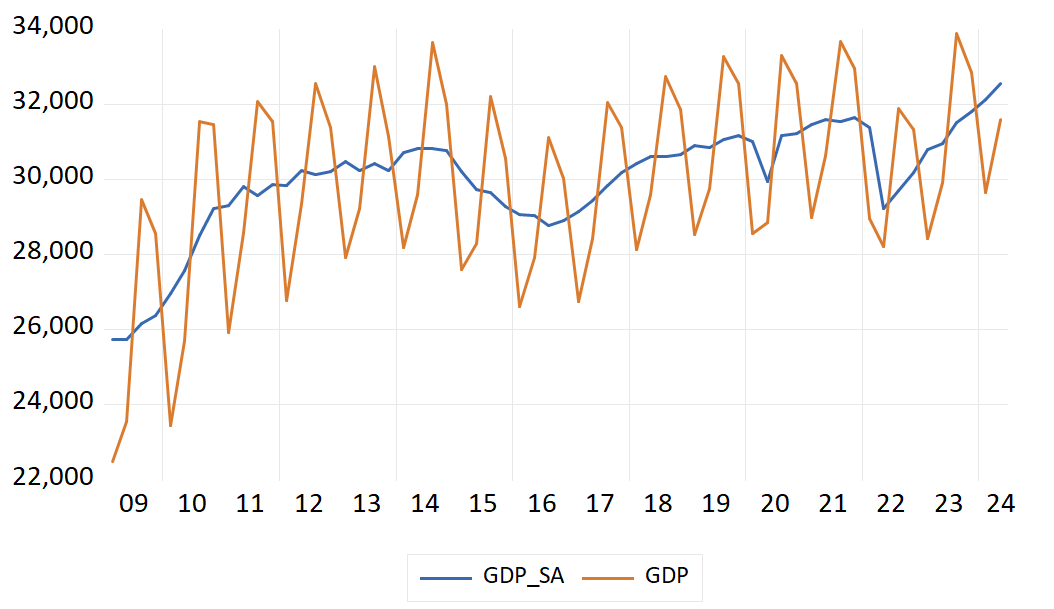
\includegraphics[scale=0.4]{images/img01}
		\caption{ВВП Беларуси (\textit{GDP}) и сезонно скорректированнный ВВП Беларуси (\textit{GDP\_SA})}
		\label{fig:img01}
	\end{figure}
	
	\begin{figure}[h]
		\centering
		\begin{minipage}{0.5\textwidth}
			\centering
		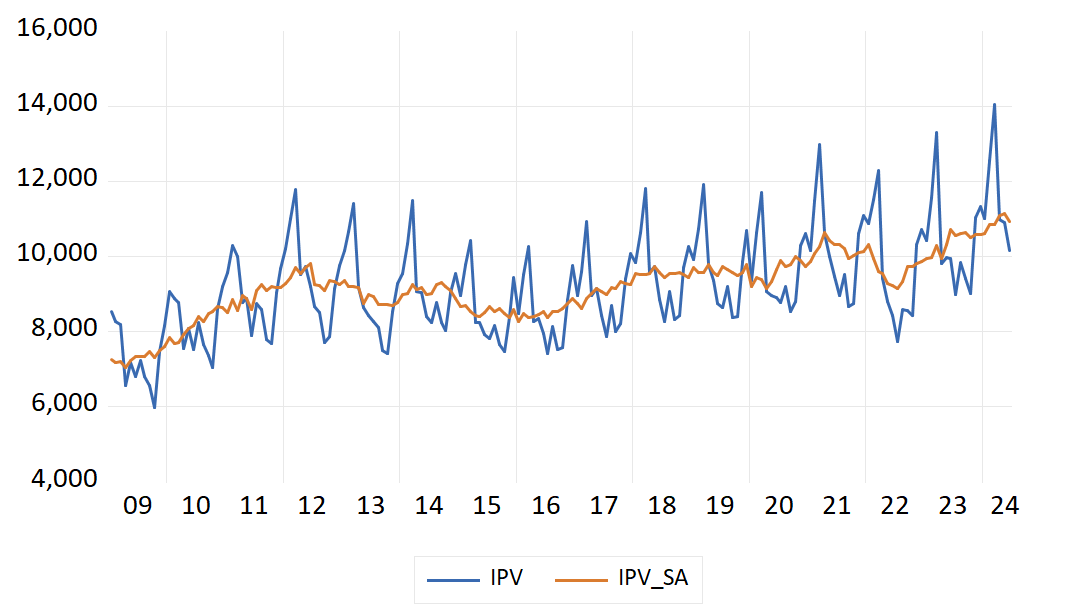
\includegraphics[scale=0.25]{images/img02}
			\caption*{а)}
		\end{minipage}%
		\begin{minipage}{0.5\textwidth}
			\centering
		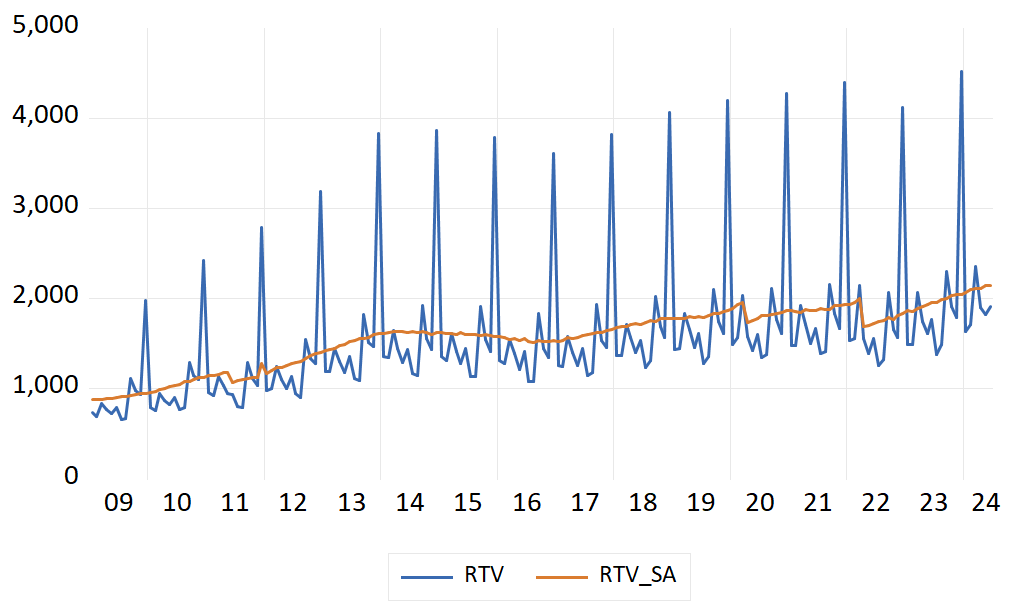
\includegraphics[scale=0.25]{images/img03}
			\caption*{б)}
		\end{minipage}%
		
		\begin{minipage}{0.5\textwidth}
			\centering
		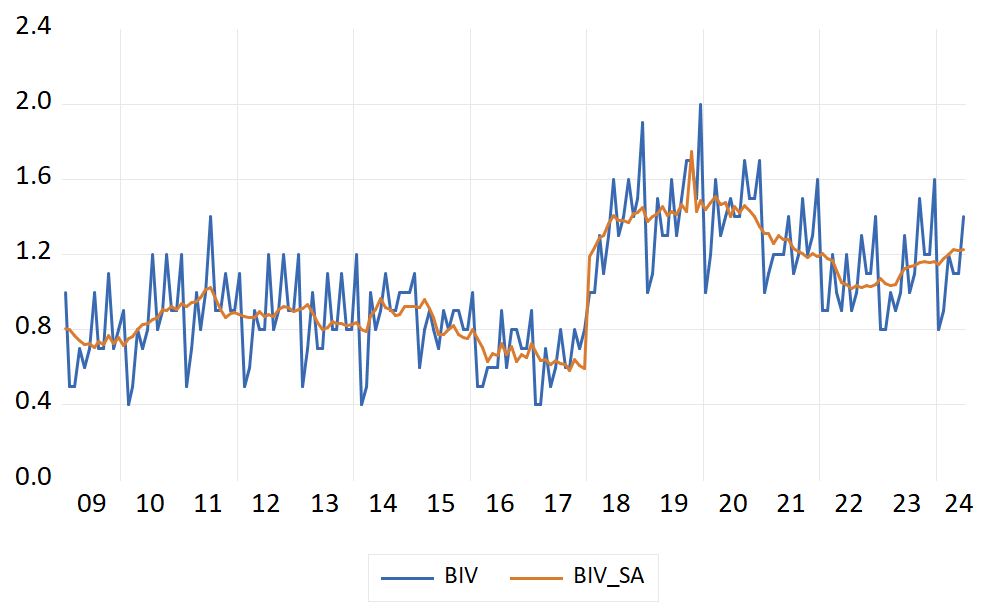
\includegraphics[scale=0.25]{images/img04}
			\caption*{в)}
		\end{minipage}%
		\hfill % Добавляем горизонтальное пространство
		\begin{minipage}{0.5\textwidth}
			\centering
		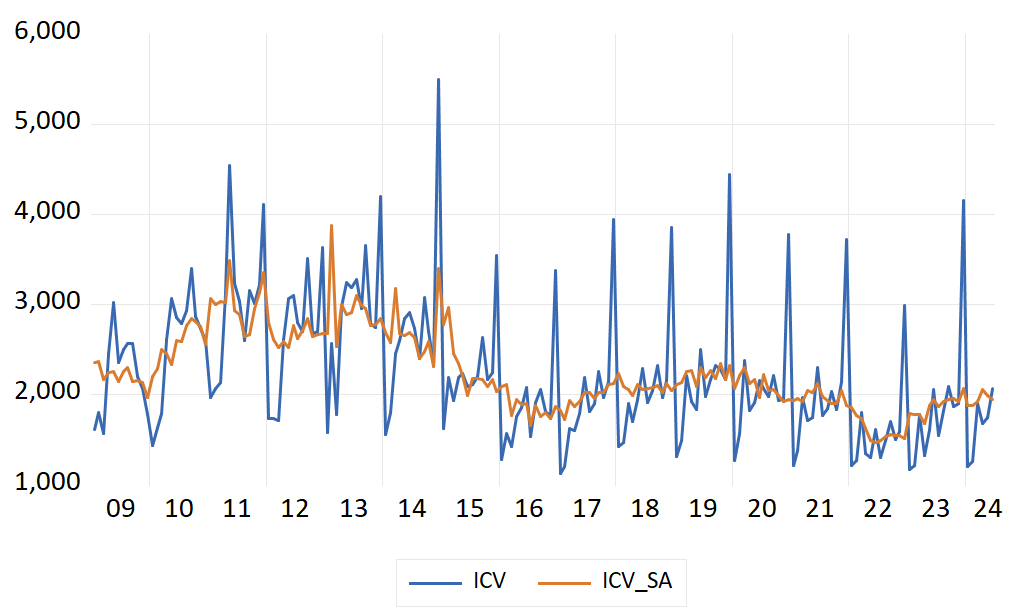
\includegraphics[scale=0.25]{images/img05}
			\caption*{г)}
		\end{minipage}%
		
		\begin{minipage}{0.5\textwidth}
			\centering
		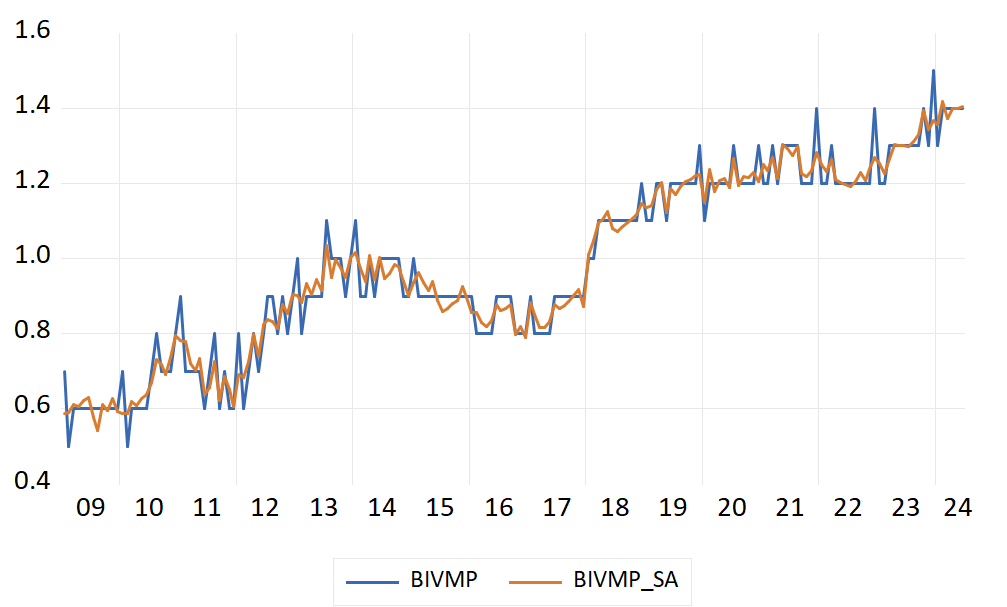
\includegraphics[scale=0.25]{images/img06}
			\caption*{д)}
		\end{minipage}%
		\hfill % Добавляем горизонтальное пространство
		\begin{minipage}{0.5\textwidth}
			\centering
		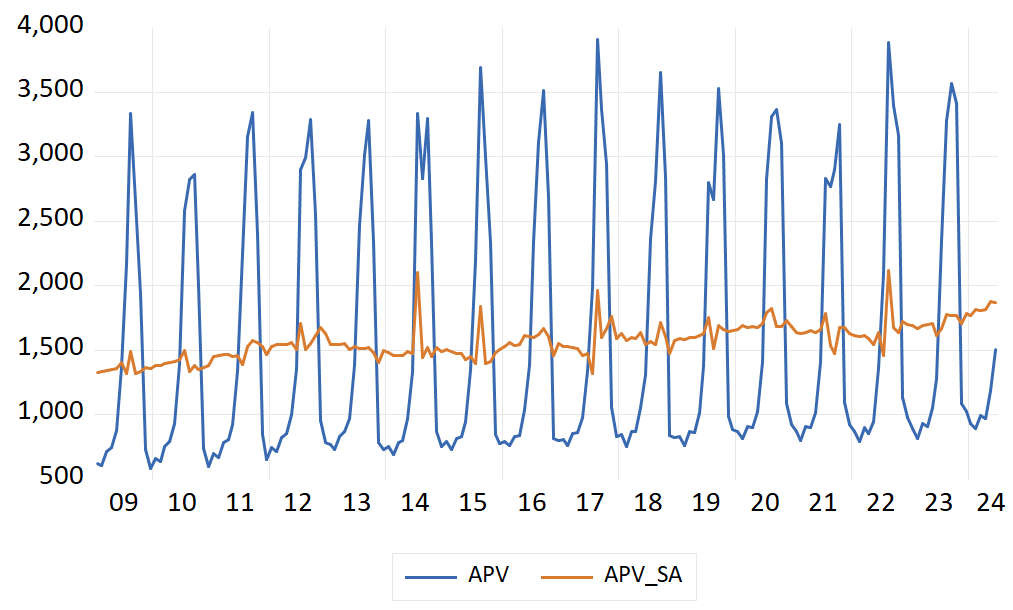
\includegraphics[scale=0.25]{images/img07}
			\caption*{е)}
		\end{minipage}
		\caption{\centering --- Исходные ряды и сезонно скорректированные:\\ а) \textit{IPV} и \textit{IPV\_SA}; б) \textit{RTV} и \textit{RTV\_SA}; в) \textit{BIV} и \textit{BIV\_SA};\\ г) \textit{ICV} и \textit{ICV\_SA}; д) \textit{BIVMP} и \textit{BIVMP\_SA}; е) \textit{APV} и \textit{APV\_SA}}
		\label{fig:sa1}
	\end{figure}
	
	Однако заметно, что в этих временных рядах все еще присутствует тренд. Поэтому следующим важным этапом будет исключение тренда.
	
	\section{Исключение тренда}
	В соответствии с \ref{greq} для исключения трендовой компоненты перейдем к темпам роста для каждого временного ряда. Переходя к темпам роста для каждого временного ряда, получим новые временные ряды
	
	\begin{equation}
		\text{GGDP\_SA}_t=\dfrac{\text{GDP\_SA}_t}{\text{GDP\_SA}_{t-1}}
	\end{equation}
	\begin{equation}
		\text{GIPV\_SA}_t=\dfrac{\text{IPV\_SA}_t}{\text{IPV\_SA}_{t-1}}
	\end{equation}
	\begin{equation}
		\text{GRTV\_SA}_t=\dfrac{\text{RTV\_SA}_t}{\text{RTV\_SA}_{t-1}}
	\end{equation}
	\begin{equation}
		\text{GICV\_SA}_t=\dfrac{\text{ICV\_SA}_t}{\text{ICV\_SA}_{t-1}}
	\end{equation}
	\begin{equation}
		\text{GBIV\_SA}_t=\dfrac{\text{BIV\_SA}_t}{\text{BIV\_SA}_{t-1}}
	\end{equation}
	\begin{equation}
		\text{GBIVMP\_SA}_t=\dfrac{\text{BIVMP\_SA}_t}{\text{BIVMP\_SA}_{t-1}}
	\end{equation}
	\begin{equation}
		\text{GAPV\_SA}_t=\dfrac{\text{APV\_SA}_t}{\text{APV\_SA}_{t-1}}
	\end{equation}
	
	Временной ряд \textit{GGDP\_SA} отражает квартальные темпы роста ВВП Беларуси (Рис. 2.3). Аналогично все месячные переменные также отображают темпы роста продукции или цен месяц к месяцу (Рис. 2.4).
	
	\begin{figure}
		\centering
		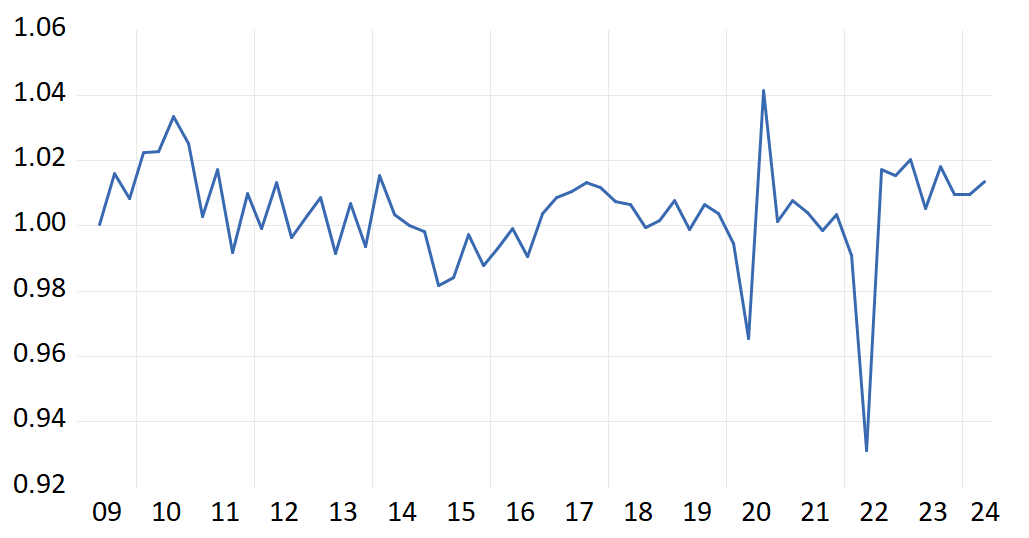
\includegraphics[scale=0.4]{images/img08}
		\caption{Темпы роста ВВП (\textit{GGDP\_SA}) квартал к кварталу}
		\label{fig:img08}
	\end{figure}
	\begin{figure}
		\centering
		\begin{minipage}{0.5\textwidth}
			\centering
		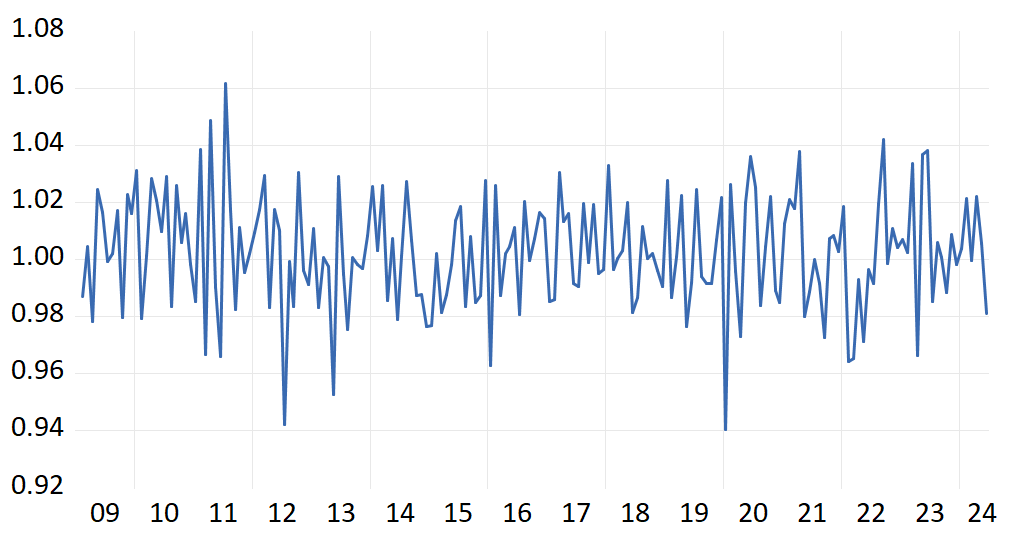
\includegraphics[scale=0.25]{images/img09}
			\caption*{а)}
		\end{minipage}%
		\begin{minipage}{0.5\textwidth}
			\centering
		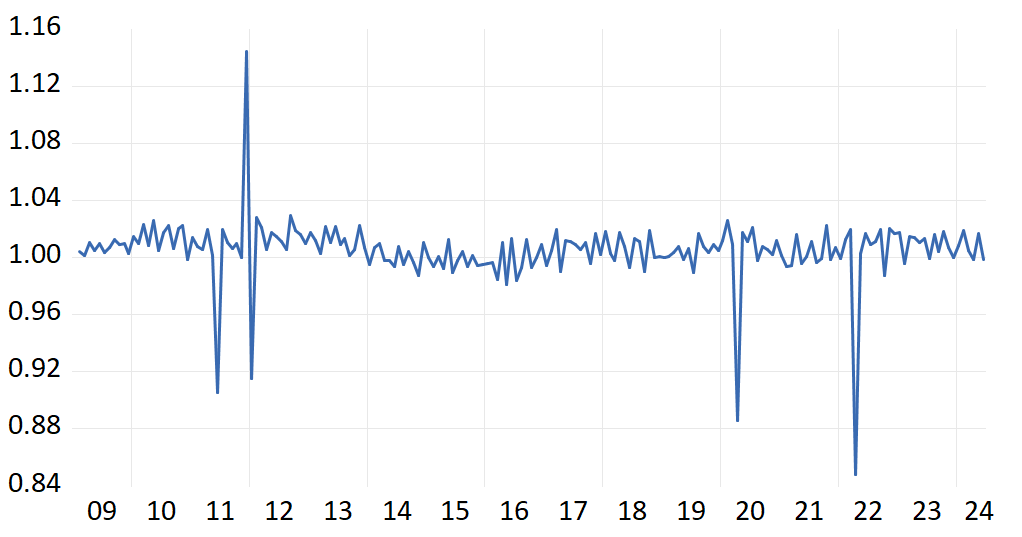
\includegraphics[scale=0.25]{images/img10}
			\caption*{б)}
		\end{minipage}%
		
		\begin{minipage}{0.5\textwidth}
			\centering
		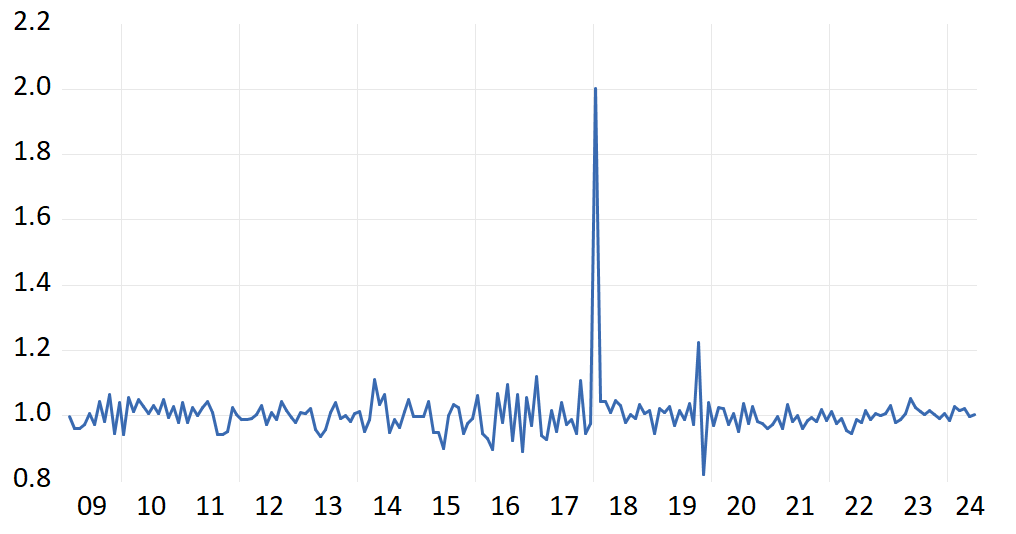
\includegraphics[scale=0.25]{images/img11}
			\caption*{в)}
		\end{minipage}%
		\hfill % Добавляем горизонтальное пространство
		\begin{minipage}{0.5\textwidth}
			\centering
		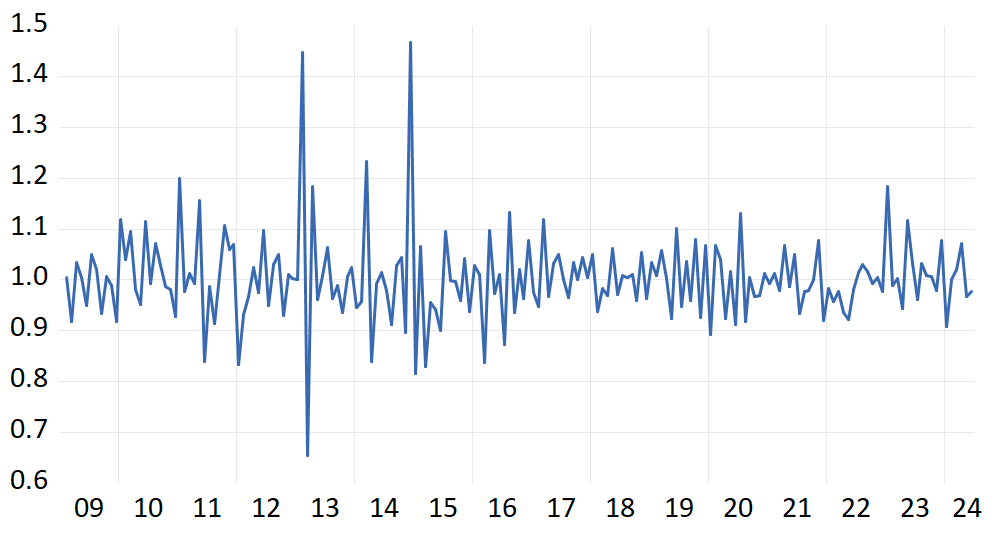
\includegraphics[scale=0.25]{images/img12}
			\caption*{г)}
		\end{minipage}%
		
		\begin{minipage}{0.5\textwidth}
			\centering
		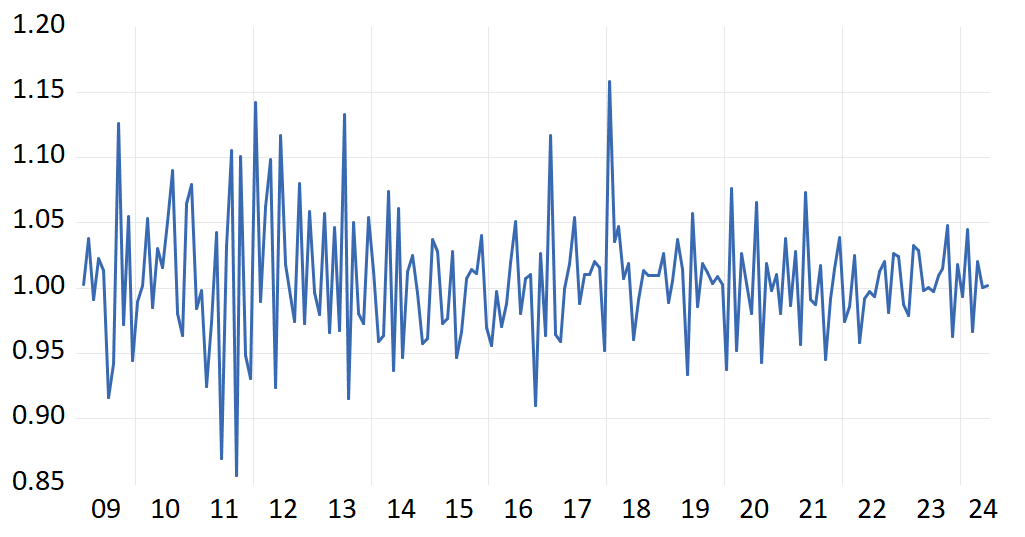
\includegraphics[scale=0.25]{images/img13}
			\caption*{д)}
		\end{minipage}%
		\hfill % Добавляем горизонтальное пространство
		\begin{minipage}{0.5\textwidth}
			\centering
		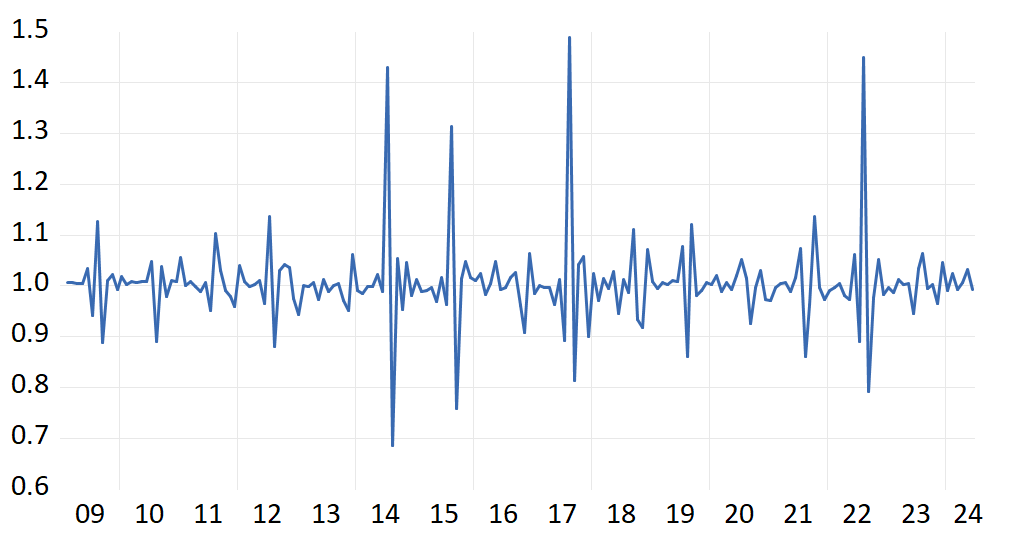
\includegraphics[scale=0.25]{images/img14}
			\caption*{е)}
		\end{minipage}
		\caption{\centering --- Темпы роста месяц к месяцу:\\ а) \textit{GIPV\_SA}; б) \textit{GRTV\_SA}; в) \textit{GBIV\_SA};\\ г) \textit{GICV\_SA}; д) \textit{GBIVMP\_SA}; е) \textit{GAPV\_SA}}
		\label{fig:gsa}
	\end{figure}
	
	Таким образом, мы получили новые временные ряды, в которых отсутствуют трендовая и сезонная компоненты. Однако этого мало для того, чтобы сделать заключение о стационарности временных рядов. Необходимо также статистически подкрепить предположения о стационарности полученных рядов, для чего мы воспользуемся тестом ADF.
	
	\section{Тестирование стационарности}
	Для тестирования стационарности и определения типа нестационарности мы проведем расширенный тест Дики-Фуллера (ADF). Этот тест является стандартным инструментом анализа временных рядов, однако следует отметить, что он может быть склонен к ошибочным выводам в случаях наличия структурных изменений, что часто приводит к предпочтению моделей с единичным корнем (DS-моделей).
	
	В связи с этой проблемой мы также применим модифицированный ADF-тест, известный как Brake Point Unit Root (BPUR-тест). Этот тест позволяет выявить одно наиболее выраженное структурное изменение во временном ряде, описываемом DS-моделью, что делает его полезным инструментом для более точного анализа.
	
	Алгоритмы работы указанных тестов и их применение подробно представлены в разделах \ref{sbs:adf} и \ref{sbs:bpur} соответственно.
	
	Таблицы \ref{adf} и \ref{bpur} содержат результаты тестирования временных рядов, проведенного с использованием тестов ADF и BPUR. Нулевая гипотеза для этих тестов формулируется следующим образом: «временной ряд является нестационарным и описывается DS-моделью». Это означает, что если нулевая гипотеза оказывается верной, то временной ряд не демонстрирует стабильности во времени и может находиться под воздействием различных структурных изменений.
	
	
	\begin{table}[h!]
		\centering
		\caption{\label{adf} -- Результаты тестирования временных рядов с помощью ADF-теста}
		\label{table:ADF-test}
		\begin{tabular}{|p{3cm}|p{3cm}|p{2.5cm}|p{2cm}|}
			\hline
			{Временной ряд} & {Значение ADF-статистики} & {Пороговые значения, $\varepsilon = 0.05$} & {Тип модели} \\ \hline
			GGDP\_SA$_t$ & -6,796  & -2,911  & TS \\ \hline
			IPV\_SAG$_t$ & -16,478 & -2,877  & TS \\ \hline
			RTV\_SAG$_t$ & -16,678 & -2,877  & TS \\ \hline
			ICV\_SAG$_t$ & -22,472 & -2,877  & TS \\ \hline
			BIV\_SAG$_t$ & -14,380 & -2,877  & TS \\ \hline
			BIVMP\_SAG$_t$ & -20,402 & -2,877 & TS \\ \hline
			APV\_SAG$_t$ & -15,410 & -2,877  & TS \\ \hline
		\end{tabular}
	\end{table}
	
	
	\begin{table}[h]
		\centering
		\caption{\label{bpur} -- Результаты тестирования временных рядов с помощью BPUR-теста}
		\label{table:BPUR-test}
		\begin{tabular}{|p{3cm}|p{3cm}|p{2.5cm}|p{3cm}|p{2cm}|}
			\hline
			{Временной ряд} & 
			{Значение ADF-статистики} & 
			{Пороговые значения, $\varepsilon = 0.05$} & 
			{Моменты структурных изменений} & 
			{Тип модели} \\ \hline
			GGDP\_SA$_t$ & -9,138  & -4,444 & 2022q2  & TS \\ \hline
			IPV\_SAG$_t$ & -17,236 & -4,444 & 2012m7  & TS \\ \hline
			RTV\_SAG$_t$ & -18,945 & -4,444 & 2022m4  & TS \\ \hline
			ICV\_SAG$_t$ & -24,902 & -4,444 & 2013m2  & TS \\ \hline
			BIV\_SAG$_t$ & -15,405 & -4,444 & 2017m1  & TS \\ \hline
			BIVMP\_SAG$_t$ & -20,985 & -4,444 & 2012m7 & TS \\ \hline
			APV\_SAG$_t$ & -24,331 & -4,444 & 2022m10 & TS \\ \hline
		\end{tabular}
	\end{table}
		
	Если статистика критерия в результате тестирования превышает установленное пороговое значение, то в таком случае нулевая гипотеза не отклоняется на уровне значимости 0,05. Это указывает на то, что временной ряд является нестационарным и, следовательно, требует применения соответствующих методов анализа. В противном случае, если статистика критерия оказывается ниже порогового значения, временной ряд считается стационарным или может быть отнесен к TS-моделям.
	
	Результаты тестирования указывают на то, что все временные ряды являются стационарными. Это означает, что их статистические свойства, такие как среднее и дисперсия, остаются постоянными во времени. Ниже приведены ключевые выводы и значения стационарности:
	\begin{enumerate}
		\item \textit{Корректность модели.} Стационарные ряды позволяют использовать модели временных рядов, включая MFVAR, без необходимости их трансформации.
		\item \textit{Прогнозирование.} Стационарные ряды обеспечивают более надёжные прогнозы благодаря предсказуемости их поведения.
		\item \textit{Стабильность взаимосвязей.} Стационарные ряды предполагают стабильность взаимосвязей между переменными, что важно для интерпретации результатов.
	\end{enumerate}
	
	\newpage
	
	\chapter{МОДЕЛИРОВАНИЕ И ПРОГНОЗИРОВАНИЕ ТЕМПОВ РОСТА ВВП БЕЛАРУСИ ПО ИСТОЧНИКАМ ДОХОДОВ}
	В данной главе будут представлены результаты прогнозирования с помощью моделей MFVAR, описанных в \ref{sec:mfvar}. В качестве низкочастотной эндогенной переменной в данной главе будет выступать сезонно скорректированные темпы роста ВВП Беларуси, полученные в предыдущей главе. Остальные же переменные будут выступать в качестве экзогенных. Причем добавлять в модель экзогенные переменные высокой частоты мы будем последовательно. Выбор порядка добавления параметров обусловлен их экономической значимостью, предсказательной силой и взаимосвязи с динамикой ВВП.
	\begin{enumerate}
		\item \textit{Темпы роста объёма промышленного производства.}
		Промышленный сектор является ключевым элементом экономики, который оказывает непосредственное влияние на формирование ВВП. Темпы
		роста объема промышленного производства отражают динамику производства товаров и услуг, что, в свою очередь, напрямую связано с объемом добавленной стоимости. Увеличение GIPV\_SA указывает на активизацию производственной деятельности, что приводит к увеличению
		ВВП в краткосрочной перспективе. Поэтому этот показатель становится
		первым в порядке добавления.
		\item \textit{Темпы роста объема розничного товарооборота}.
		Розничный товарооборот является индикатором потребительского спроса и активности в сфере услуг. Он отражает уровень потребления домохозяйств и может служить предвестником экономической активности.
		Увеличение розничных продаж часто ведет к росту производства и, как
		следствие, к росту ВВП.
		\item \textit{Темпы роста объема сельскохозяйственных работ}.
		Сельское хозяйство играет значительную роль в экономике Беларуси, однако его влияние на ВВП может быть менее предсказуемым в краткосрочной перспективе. Темпы роста объема сельскохозяйственных работ могут
		колебаться из-за сезонных факторов и погодных условий. Тем не менее рост в этом секторе может позитивно сказаться на ВВП.
		\item \textit{Темпы роста строительно-монтажных работ}.
		Строительство является важным драйвером экономического роста, так
		как этот сектор создает рабочие места и способствует инвестициям. Темпы роста объема строительно-монтажных работ могут служить индикатором будущих экономических изменений, так как рост в строительстве
		часто предшествует увеличению экономической активности в других секторах.
		\item \textit{Темпы роста доходов населения}.
		Темпы роста доходов населения влияют на потребление и инвестиции,
		однако они могут проявлять свою предсказательную силу с некоторым
		запаздыванием. Повышение доходов может способствовать увеличению
		потребительского спроса, что положительно сказывается на росте ВВП.
		\item \textit{Темпы роста инвестиций в основной капитал}.
		Инвестиции в основной капитал являются важным индикатором долгосрочного экономического роста, но их краткосрочная предсказательная
		сила может быть ограниченной. Хотя инвестиции могут способствовать
		росту производительных мощностей и, следовательно, ВВП в долгосрочной перспективе, их влияние на краткосрочные изменения в ВВП может
		быть менее заметным. 
	\end{enumerate}
	
	Помимо вышеперечисленных переменных мы также в качестве экзогенной переменной добавим фиктивную переменную с квартальной частотой DUM2022Q2. Так как из Таблицы 2.2 можно увидеть, что момент 2022q2 является моментом структурных изменений, что может сильно сказаться на прогнозах. Поэтому мы добавляем переменную, которая принимает на каждом квартале значение 0, а на 2-ом квартале 2022-ого года -- значение 1.
	
	В соответствии с методологией построения наукастов, прогнозы мы будем строить по описанному в \ref{sec:methods} алгоритму: исключать последний квартал из обучающей выборки, обучать модель, а затем оценивать модель оп последним 12 точкам и отдельно по 13-ой вневыборочной точке.
	
	MFVAR модели также требуют от исследователя задать количество лагов. Ниже будут представлены модели с заранее определенным количеством лагом, основанном на сравнении метрик. То есть будет выбрано такое число лагов, при котором значение метрик наилучшее.
	\section{MFVAR на основе промышленности, товарооборота и сельского хозяйства}
	Для построения MFVAR модели в качестве экзогенных выступали
	переменные GIPV\_SA (промышленность), GRTV\_SA (товарооборот), GAPV\_SA (сельское хозяйство), а также дамми-переменная
	DUM2022q2, а в качестве эндогенной переменной - GGDP\_SA. 
	
	Число лагов выберем равное 4.
	
	Результаты построения модели
	иллюстрируется на Рис.3.1.
	
	\begin{figure}[h]
		\centering
		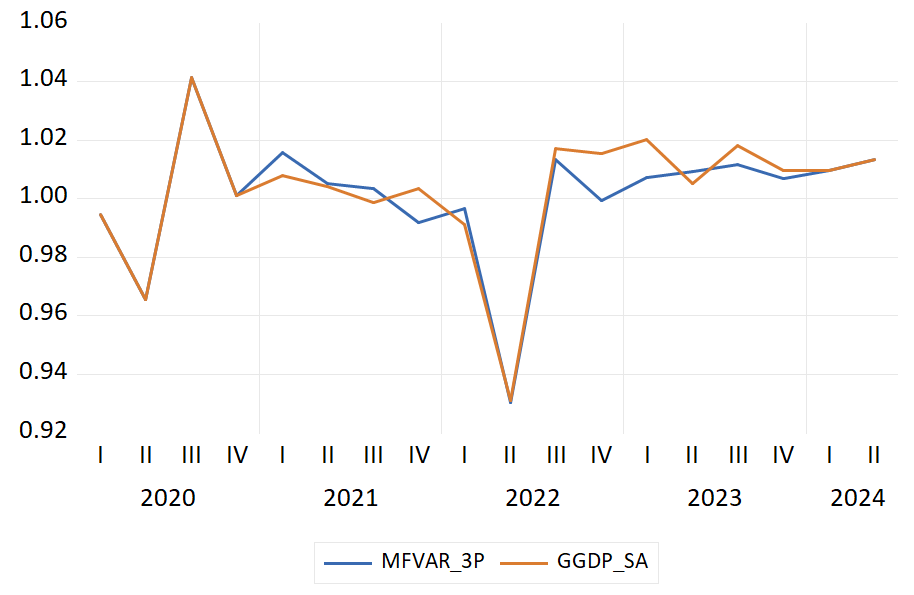
\includegraphics[scale=0.5]{images/img15}
		\caption{Ретроспективный прогноз модели MFVAR по 3 параметрам}
		\label{fig:img15}
	\end{figure}
	
	Рассмотрим поведение остатков модели на наличие закономерностей на Рис. 3.2.
	
	\begin{figure}[h!]
		\centering
		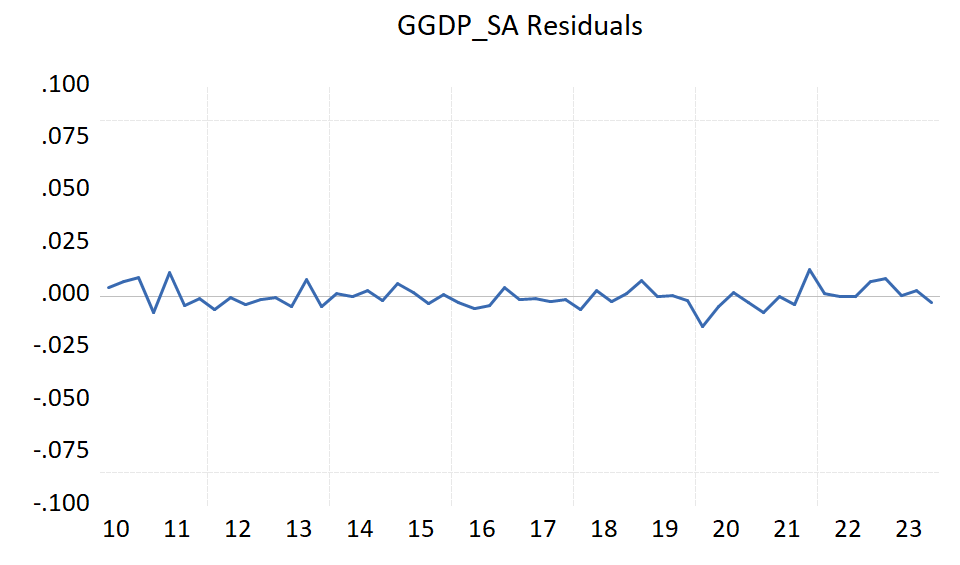
\includegraphics[scale=0.5]{images/img16}
		\caption{Остатки модели MFVAR по 3 параметрам}
		\label{fig:img16}
	\end{figure}
	
	Как можно видеть, никаких явных закономерностей нет, поэтому мы можем считать построенную MFVAR модель адекватной для прогнозирования.
	
	\section{MFVAR на основе промышленности, товарооборота сельского хозяйства, строительства}
	Для построения MFVAR модели в качестве экзогенных выступали
	переменные GIPV\_SA (промышленность), GRTV\_SA (товарооборот), GAPV\_SA (сельское хозяйство), GBIV\_SA (строительство) а также дамми-переменная
	DUM2022q2, а в качестве эндогенной переменной -- GGDP\_SA. 
	
	Число лагов выберем равное 4.
	
	Результаты построения модели
	иллюстрируется на Рис.3.3.
	
	\begin{figure}[h]
		\centering
		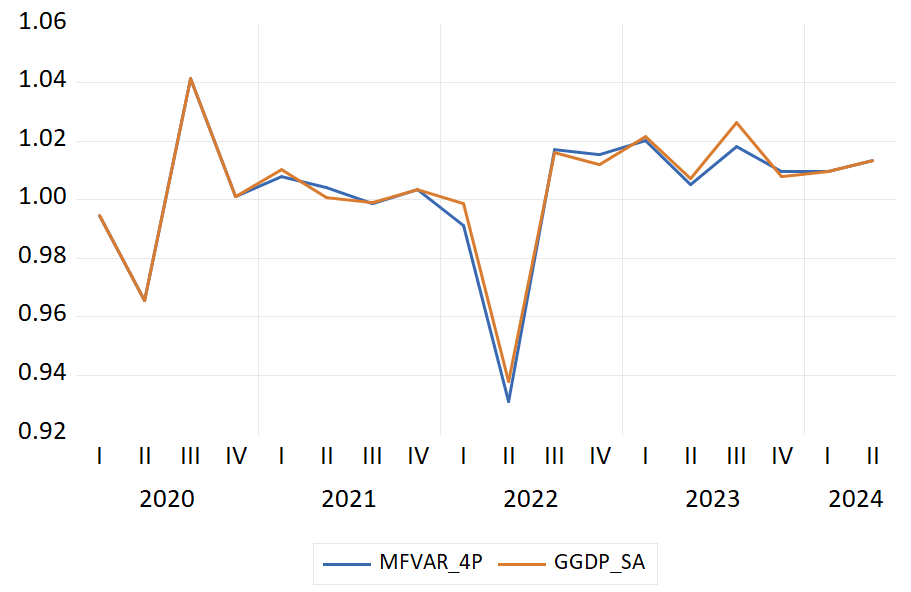
\includegraphics[scale=0.5]{images/img17}
		\caption{Ретроспективный прогноз модели MFVAR по 4 параметрам}
		\label{fig:img17}
	\end{figure}
	
	Рассмотрим поведение остатков модели на наличие закономерностей на Рис. 3.4.
	
	\begin{figure}[h!]
		\centering
		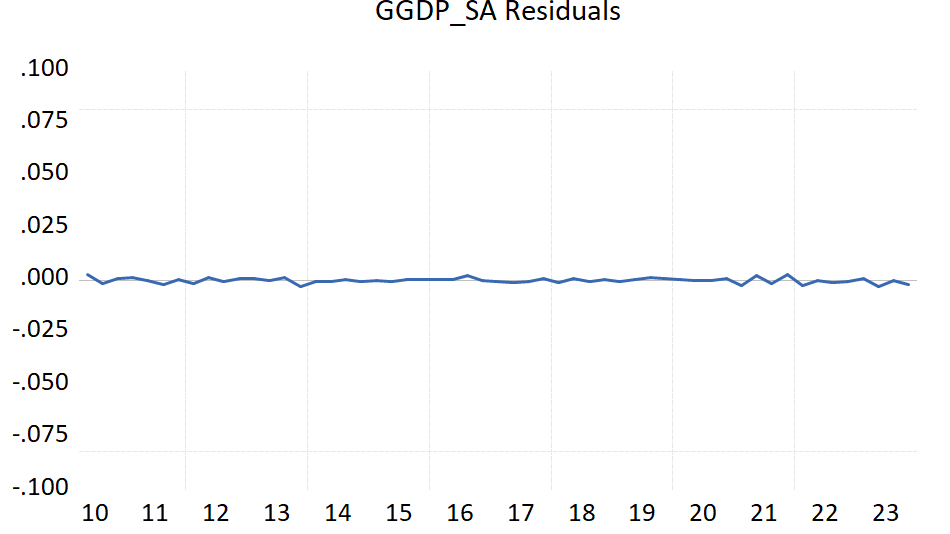
\includegraphics[scale=0.5]{images/img18}
		\caption{Остатки модели MFVAR по 4 параметрам}
		\label{fig:img18}
	\end{figure}
	
	Как можно видеть, никаких явных закономерностей нет, поэтому мы можем считать построенную MFVAR модель адекватной для прогнозирования.
	
	\section{MFVAR на основе промышленности, товарооборота, сельского хозяйства, строительства, объема инвестиций}
	Для построения MFVAR модели в качестве экзогенных выступали
	переменные GIPV\_SA (промышленность), GRTV\_SA (товарооборот), GAPV\_SA (сельское хозяйство), GBIV\_SA (строительство), GICV\_SA (объем инвестиций), а также дамми-переменная
	DUM2022q2, а в качестве эндогенной переменной -- GGDP\_SA. 
	
	Число лагов выберем равное 3.
	
	Результаты построения модели
	иллюстрируется на Рис. 3.5.
	
	\begin{figure}[h]
		\centering
		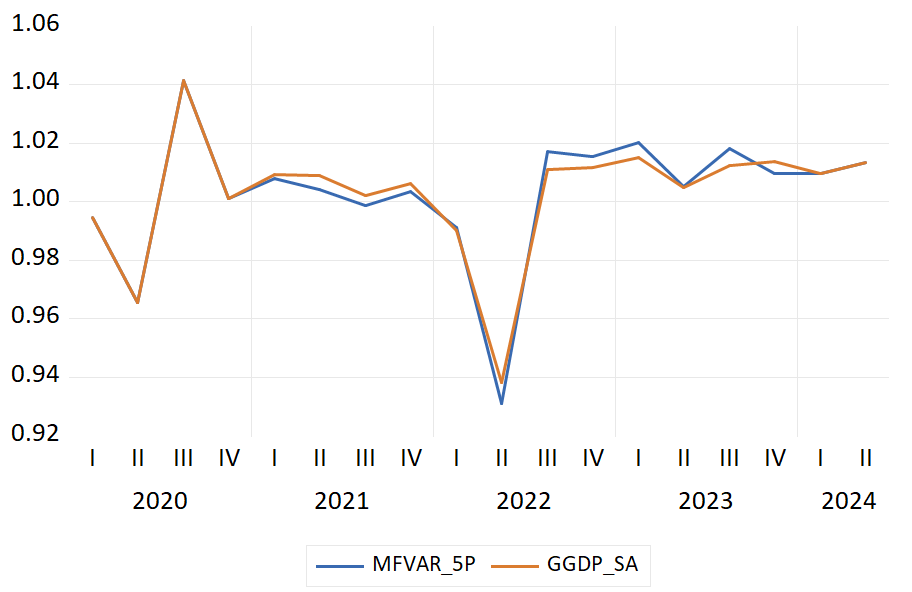
\includegraphics[scale=0.45]{images/img19}
		\caption{Ретроспективный прогноз модели MFVAR по 5 параметрам}
		\label{fig:img19}
	\end{figure}
	
	Рассмотрим поведение остатков модели на наличие закономерностей на Рис. 3.6.
	
	\begin{figure}[h!]
		\centering
		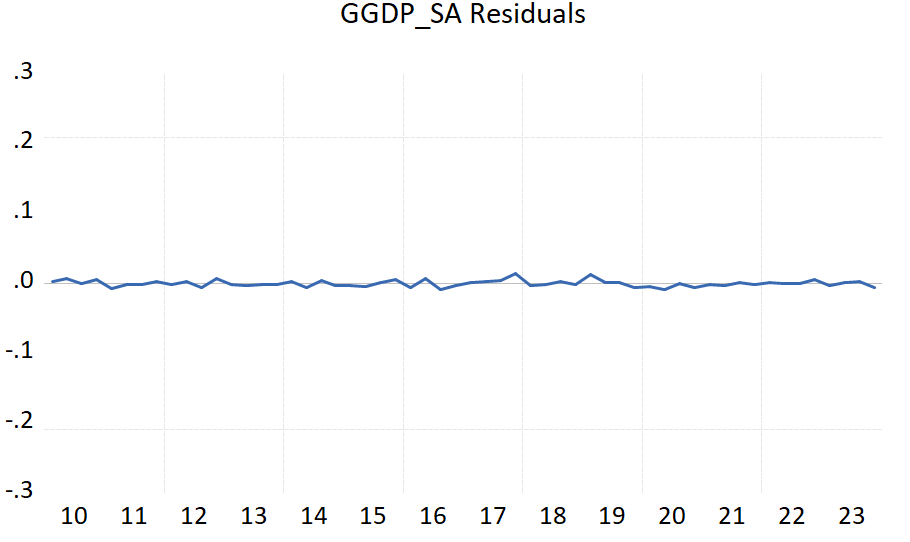
\includegraphics[scale=0.45]{images/img20}
		\caption{Остатки модели MFVAR по 5 параметрам}
		\label{fig:img20}
	\end{figure}
	
	Как можно видеть, никаких явных закономерностей нет, поэтому мы можем считать построенную MFVAR модель адекватной для прогнозирования.
	
	\section{MFVAR на основе промышленности, товарооборота, сельского хозяйства, строительства, объема инвестиций, доходов населения}
	
	Для построения MFVAR модели в качестве экзогенных выступали
	переменные GIPV\_SA (промышленность), GRTV\_SA (товарооборот), GAPV\_SA (сельское хозяйство), GBIV\_SA (строительство), GICV\_SA (объем инвестиций), GBIVM\_SA (доходы населения), а также дамми-переменная\\
	DUM2022q2, а в качестве эндогенной переменной -- GGDP\_SA. 
	
	Число лагов выберем равное 2.
	
	Результаты построения модели
	иллюстрируется на Рис.3.7.
	
	\begin{figure}[h]
		\centering
		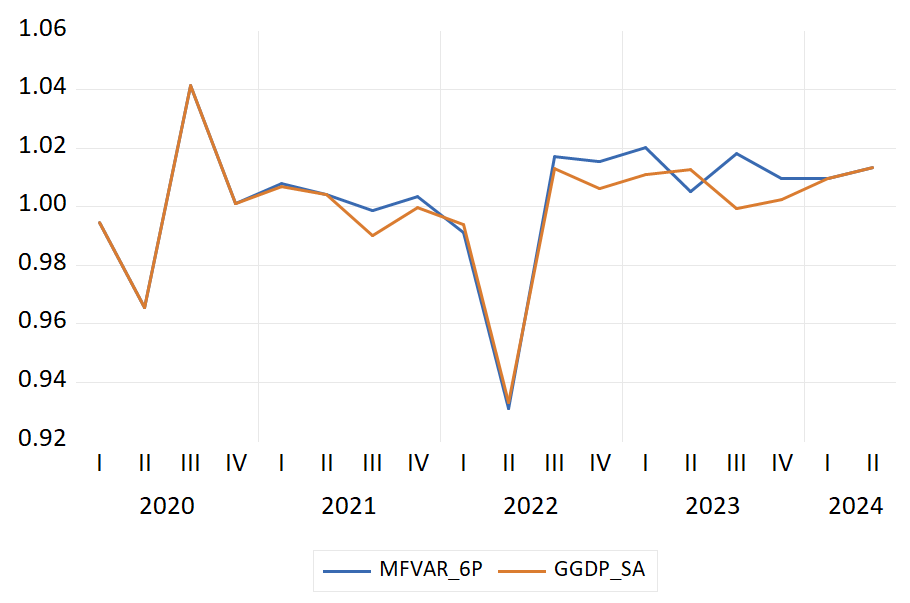
\includegraphics[scale=0.5]{images/img21}
		\caption{Ретроспективный прогноз модели MFVAR по 6 параметрам}
		\label{fig:img21}
	\end{figure}
	
	Рассмотрим поведение остатков модели на наличие закономерностей на Рис. 3.8.
	
	\begin{figure}[h!]
		\centering
		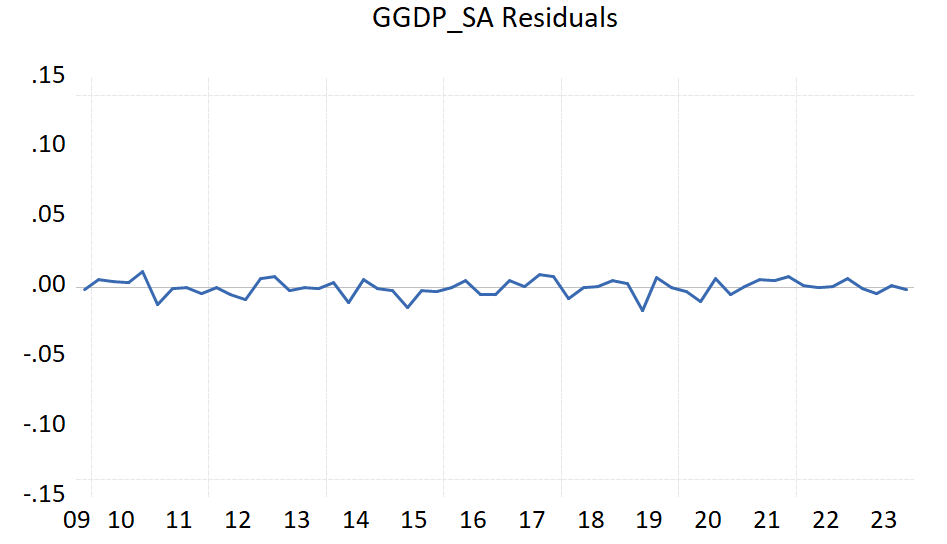
\includegraphics[scale=0.5]{images/img22}
		\caption{Остатки модели MFVAR по 6 параметрам}
		\label{fig:img22}
	\end{figure}
	
	Как можно видеть, никаких явных закономерностей нет, поэтому мы можем считать построенную MFVAR модель адекватной для прогнозирования.
	\newpage
	\section{Оценки моделей и сравнительный анализ}
	Таким образом, мы построили MFVAR модели и проделали с помощью них ретроспективные прогнозы. Теперь проделаем сам наукаст: спрогнозируем значение на следующий квартал и оценим его точность, а затем сравним результаты.
	
	\begin{figure}[h!]
		\centering
		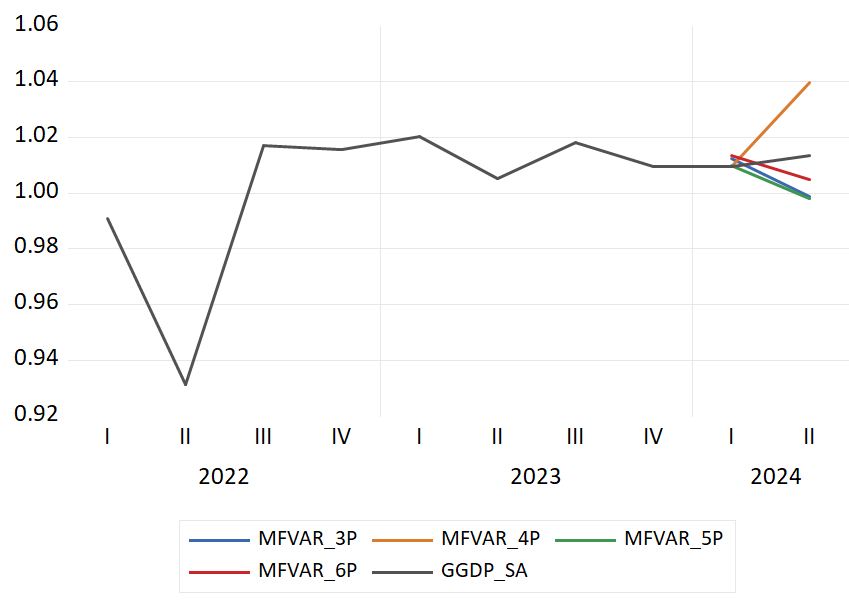
\includegraphics[scale=0.5]{images/img23}
		\caption{Краткосрочные прогнозы всех MFVAR моделей на вневыборочном квартале}
		\label{fig:img23}
	\end{figure}
	
	Заметно, что большинство моделей спрогнозировало спад ВВП, но четырехпараметрическая модель наоборт спрогнозировала сильный рост.
	
	Рассмотрим таблицу с оценками всех указанных моделей и сделаем на основании этого выводы.
	
\begin{table}[h!]
	\caption{\label{toch}\centering --- Показатели точности прогнозов годовых темпов роста ВВП РБ на основе альтернативных моделей, период оценивания моделей: 2021q1-2023q4}
	\begin{center}
		\begin{tabular}{|c|c|c|c|c|c|}
			\hline\multicolumn{6}{|c|}{\vspace{-0.5em}}\\
			\multicolumn{6}{|c|}{Прогнозный период: 2021q1 – 2023q4 (ретроспективные прогнозы)}\\
			\multicolumn{6}{|c|}{\vspace{-0.6em}}\\
			\hline
			Модель & \specialcell{Число\\наблюдений} & RMSE & MAE & MAPE,\ \% & Lag\\
			\hline
			MFVAR\_3P & 12 &  0.007958 &  0.006491 &  0.647089 & 4\\
			\hline
			MFVAR\_4P& 12 &  0.004152
			 &  0.003195
			  &  0.320232
			  & 4 \\
			\hline
			MFVAR\_5P& 12 &  0.004336
			 &  0.003847
			  &  0.385297
			   & 3\\
			\hline
			MFVAR\_6P& 12 &  0.007863
			 &  0.006145
			  &  0.613890
			   & 2\\
			\hline\multicolumn{6}{|c|}{\vspace{-0.5em}}\\
			\multicolumn{6}{|c|}{\specialcell{Прогнозный период: 2024q1 – 2024q2\\ (краткосрочный прогноз)}}\\
			\multicolumn{6}{|c|}{\vspace{-0.6em}}\\
			\hline
			MFVAR\_3P& 2 &  0.010541
			 &  0.008671
			  &  0.866359
			   & 4\\
			\hline
			MFVAR\_4P& 2 &  0.018522
			 &  0.013152
			  &  1.265229
			   & 4\\
			\hline
			MFVAR\_5P& 2 &  0.010820
			 &  0.007860
			  &  0.787171
			   & 3\\
			\hline
			MFVAR\_6P& 2 &  0.006649
			 &  0.006215
			  &  0.616806
			   & 2\\
			\hline
		\end{tabular}
	\end{center}
\end{table}

Исходя из данных таблицы можем сделать следующие выводы:
\begin{itemize}
	\item по оценкам RMSE и MAPE на ретроспективном прогнозе лучше всех оказалась модель с 4 переменными;
	\item по оценкам RMSE и  MAPE на краткосрочном прогнозе лучше всех оказалась модель с 6 переменными, которая спрогнозировала самый слабы спад относительно всех остальных моделей.
\end{itemize}
	
	\newpage
	\chapter*{ЗАКЛЮЧЕНИЕ}\addcontentsline{toc}{chapter}{ЗАКЛЮЧЕНИЕ}
	В данной работе была рассмотрена задача прогнозирования компонент ВВП на основе регрессионных моделей MFVAR. В ходе исследования
	\begin{enumerate}
		\item было дано теоретическое описание всех используемых для решения данной задачи моделей;
		\item были рассмотрены свойства и особенности, которые возникают в ходе работы с исследуемыми моделями;
		\item был проведен полный цикл исследования и преобразования моделей временных рядов для приведения к стационарному виду;
		\item были построены модели MFVAR для прогнозирования и оценки темпов роста ВВП Беларуси по его компонентам, такиим как объем промышленности, объем товарооборота, сельского хозяйства, объем строительства, объем инвестиций, объем доходов населения;
		\item был проведен сравнительный анализ точности прогнозных значений и ретроспективных прогнозов моделей MFVAR в зависимости от переменных.
	\end{enumerate}
	Таким образом, данная работа вносит вклад в развитие методов прогнозирования на основе моделей временных рядов по смешанным данных и
	может быть использована в дальнейших исследованиях и практических применениях в области экономики и финансов.
	\newpage
	\chapter*{СПИСОК ИСТОЧНИКОВ}\addcontentsline{toc}{chapter}{СПИСОК ИСПОЛЬЗОВАННОЙ ЛИТЕРАТУРЫ}
	\begin{enumerate}
		\item Тест Дики — Фуллера. [Электронный ресурс] – \texttt{https://ru.wikipedia.\\org/wiki/Тест\_Дики\_—\_Фуллера} – Дата доступа: 02.11.2024.
		\item Понятие стационарности временного ряда. Процессы «единичного корня».
		[Электронный ресурс] – \texttt{https://bsu.by/upload/page/544153\\.pdf} – Дата
		доступа: 02.11.2024
		\item Процессы «единичного корня».
		Тесты «единичного корня»: ADF, PP, KPSS.
		[Электронный ресурс] – \texttt{https://bsu.by/upload/page/546923.\\pdf} – Дата
		доступа: 02.11.2024
		\item Харин, Ю. С. Теория вероятностей,
		математическая
		и прикладная статистика / Ю. С. Харин, Н. М. Зуев, Е. Е. Жук // Минск : БГУ, 2011. 
		\item Интерактивная информационно-аналитическая система распространения
		официальной статистической информации. [Электронный ресурс] – \texttt{https:
		//dataportal.belstat.gov.by/} – Дата доступа: \\ 02.12.2024.
		\item Макеева, Н.М., Наукастинг элементов использования ВВП России / Н.М. Макеева, И.П. Станкевич // Статья 2022/10, Экономический журнал ВШЭ.
		\item Станкевич И.П. Сравнение методов наукастинга макроэкономических индикаторов на примере российского ВВП // Прикладная эконометрика 2020. С. 113–127.
		\item Малюгин, В. Краткосрочное прогнозирование и наукастинг темпов роста инфляции на основе моделей по смешанным данным / В.И. Малюгин // Банкаўскі веснік. – 2024. – С. 1–13.
		\item Ghysels, E. Regression models with mixed sampling frequencies /  E. Andreou, A. Kourtellos // Journal of Econometrics 2010.
		\item Soybilgen, B. Nowcasting the New Turkish GDP / B. Soybilgen, E. Yazgan // Economics Bulletin, Volume 38, Issue 2, 
		С. 1083-1089
		\item Kuzin, V. MIDAS vs. Mixed-Frequency VAR:
		Nowcasting GDP in the Euro Area / V. Kuzin,
		M. Marcellino, C. Shumacher // EUI Working Paper.
		\item X-13ARIMA-SEATS. [Электронный ресурс] – \texttt{https://en.wikipedia.
		org/wiki/X-13ARIMA-SEATS} – Дата доступа: 26.11.2024.
		\item «Сгладить нельзя не сгладить!» или пара слов о том, как строить
		свои отношения с сезонностью в данных. [Электронный ресурс] –
		\texttt{https://www.econ.msu.ru/ext/lib/Category/x81/xf9/33273/file\\/Встреча\%207\_\%20Сезонность.pdf} – Дата доступа:
		26.11.2024.
		\item Perron, P. Testing for a Unit Root in a Time Series with a Changing Mean. –
		Journal of Business and Economic Statistics, Volume 8, Issue 2. – pp. 153–162.
		\item Perron, P. A Note on the Additive Outlier Model with Breaks. / Perron, P.,
		Vogelsang, T.J. – Revista de Econometria Volume 13. – pp. 181–201.
		\item Perron, P. The Great Crash, the Oil Price Shock and the Unit Root
		Hypothesis: Erratum / Perron, P., Vogelsang, T.J. – Econometrica, Volume 61.
		– pp. 248–249.
	\end{enumerate}
	
\end{document}